\documentclass{article}

\usepackage{geometry}
\usepackage{makecell}
\usepackage{array}
\usepackage{multicol}
\usepackage{setspace}
\usepackage{changepage}
\usepackage{nicefrac}
\usepackage{amssymb}
\usepackage{amsmath}
\usepackage{cancel}
\usepackage{stmaryrd}
\usepackage{polynom}
\usepackage{booktabs}
\usepackage[explicit]{titlesec}
\usepackage{hyperref}
\usepackage{graphicx}
\usepackage{cprotect}
\usepackage{float}
\usepackage{enumitem}
\newcolumntype{?}{!{\vrule width 1pt}}
\newcommand{\paragraphlb}[1]{\paragraph{#1}\mbox{}\\}
\newcommand{\subparagraphlb}[1]{\subparagraph{#1}\mbox{}\\}
\renewcommand{\contentsname}{Inhaltsverzeichnis:}
\renewcommand\theadalign{tl}


\newcommand{\N}{\mathbb{N}}
\newcommand{\Z}{\mathbb{Z}}
\newcommand{\Q}{\mathbb{Q}}
\newcommand{\R}{\mathbb{R}}
\newcommand{\M}{\mathbb{M}}
\setstretch{1.10}
\setlength{\parindent}{0pt}
\setcounter{tocdepth}{5}

\titleformat{\section}
  {\normalfont\Large\bfseries}{\thesection}{1em}{\hyperlink{sec-\thesection}{#1}
\addtocontents{toc}{\protect\hypertarget{sec-\thesection}{}}}
\titleformat{name=\section,numberless}
  {\normalfont\Large\bfseries}{}{0pt}{#1}

\titleformat{\subsection}
  {\normalfont\large\bfseries}{\thesubsection}{1em}{\hyperlink{subsec-\thesubsection}{#1}
\addtocontents{toc}{\protect\hypertarget{subsec-\thesubsection}{}}}
\titleformat{name=\subsection,numberless}
  {\normalfont\large\bfseries}{\thesubsection}{0pt}{#1}

\hypersetup{
    colorlinks,
    citecolor=black,
    filecolor=black,
    linkcolor=black,
    urlcolor=black
}

\geometry{top=12mm, left=1cm, right=2cm}
\title{\vspace{-1cm}Mathematik für Informatik 2 - Übungen}
\author{Andreas Hofer}

\begin{document}
	\maketitle
	\tableofcontents
	\section{Kombinatorik}
	\begin{itemize}
		\item[2]{Wie viele verschiedene 4-stellige PINS lassen sich aus folgenden Ziffern bilden, wenn man jede der Ziffern auch mehr als einmal vorkommen darf?}
		\begin{itemize}
			\item[a)]{0, 1, 2}
			\begin{itemize}
				\item{Die Maske ist ZZZZ wobei jede Möglichkeit 0, 1 oder 2 sein kann. Hierbei muss man die Produktregel anwenden: $n^k=3^4=81$}
			\end{itemize}
			\item[b)]{3, 5, 6, 9}
			\begin{itemize}
				\item{Gleiche Maske von ZZZZ jedoch mit 4 Möglichkeiten: $4^4=256$}
			\end{itemize}
			\item[c)]{1, 3, 5, 6, 9}
			\begin{itemize}
				\item{Wieder ZZZZ mit 5 Möglichkeiten: $5^4=625$}
			\end{itemize}
		\end{itemize}
		\item[3]{Ein Kleidungshersteller bietet Jeans in fünf verschiedenen Größen, vier verschiedenen Farben und in drei unterchiedlichen Schnitten an. Wie viele unterschiedliche Jeans gibt es?}
		\begin{itemize}
			\item{Da jede der drei Teilmöglichkeiten unabhängig sind, muss man wieder die Produktregel anwenden: $5*4*3=60$}
		\end{itemize}
		\item[4]{Es wird 3 Mal gewürfelt und die Augenzahlen werden nebeneinander aufgeschrieben.}
		\begin{itemize}
			\item[a]{Wie viele verschiedene 3-stellige Zahlen sind dabei möglich?}
			\begin{itemize}
				\item{Es gibt drei Möglichkeiten, weshalb die Maske wie ZZZ aussieht. Da es 6 Möglichkeiten gibt, ist die Formel $n^k=6^3=216$}
			\end{itemize}
			\item[b]{Wie viele verschiedene gerade 3-stellige Zahlen sind dabei möglich?}
			\begin{itemize}
				\item{Da die Zahl nur Gerade ist, wenn die letzte Ziffer gerade ist, kann man die Maske als ZZG aufschreiben, während G jeweils eine gerade Zahl ist. Die Formel lautet also $6*6*3=6^2*3=108$}
			\end{itemize}
		\end{itemize}
		\item[6]{Wie viele verschiedene Wörter (auch sinnfreie) aus Kleinbuchstaben der Länge 3, 4 oder 5 gibt es?}
		\begin{itemize}
			\item{$26^3+26^4+26^5=12.355.928$}
		\end{itemize}
		\item[7]{Wie viele verschiedene 6-stellige Passwörter können aus Groß- und Kleinbuchstaben, Ziffern und Sonderzeichen \verb|!?.;:<>#| gebildet werden?}
		\begin{itemize}
			\item{Man hat 26 Klein- und Großbuchstaben, sowie 10 Ziffern und 8 Sonderzeichen, wodurch man zu 70 Möglichkeiten kommt. Bei 6 Stellen berechnet man so $70^6=117.649.000.000$ Möglichkeiten}
		\end{itemize}
		\item[8]{Wie viele verschieden Wörter (auch sinnfreie) aus 3 Kleinbuchstaben, die mit einem Vokal (a,e,i,o,u) beginnen oder einem Vokal enden, gibt es?}
		\begin{itemize}
			\item{Da ein Wort, welches mit einem Vokal beginnt, auch mit einem Vokal enden kann, muss man beide Teile kombinieren und danach die Schnittmenge abziehen: $5*26^2+26^2*5-5*26*5=3380+3380-650=6110$}
		\end{itemize}
		\item[13]{In einer Fußballliga gibt es 16 Mannschaften. Wie viele Spiele finden insgesamt in einer Saison statt, wenn es zwischen zwei Mannschaften je ein Hin- und ein Rückspiel gibt?}
		\begin{itemize}
			\item{Die Reihenfolge ist relevant, da zwei Mannschaften jeweils in zwei Konstellationen gegeneinander spielen sollen und ohne Zurücklegen, da keine Mannschaft gegen sich selbst spielen soll. $\frac{n!}{(n-k)!}=\frac{16!}{(16-2)!}=\frac{16!}{14!}=\frac{16*15*\cancel{14!}}{\cancel{14!}}=16*15=240$}
			\item{Ein Alternativer Lösungsweg ist, keine Reihenfolge zu verwenden wodurch man nur die Anzahl der Paarungen der Mannschaften berechnet. Wenn man diese danach mit 2 multipliziert, erhält man das selbe Ergebnis.}
		\end{itemize}
		\item[14]{In einem Schulfach gibt es ein Schulübungsheft und ein Hausübungsheft. Wie viele Möglichkeiten gibt es, die Hefte einzubinden, wenn es Heftumschläge in 8 verschiedenen Farben gibt und folgende Richtlinien eingehalten werden.}
		\begin{itemize}
			\item[a)]{Hefte sollen unterschiedliche Farben haben}
			\begin{itemize}
				\item{Mit Reihenfolge, ohne Zurücklegen: $\frac{n!}{(n-k)!}$}
			\end{itemize}
		\end{itemize}
		\item[17]{Wie viele Möglichkeiten gibt es, aus 2 blauen und 3 grünen Bausteinen, die sich nur durch Farbe unterscheiden, einen 4 Steine hohen Turm zu bauen?}
		\begin{itemize}
			\item{Da jeder Turm aus mindestens zwei Farben bestehen muss, muss man dieses Beispiel in zwei Phasen berechnen: Zuerst mit einem blauen und danach mit zwei blauen Steinen.}
			\item{Da alle grünen Steine ununterscheidbar sind und man jeden Stein nur ein Mal ziehen will, berechnet man es ohne Reihenfolge und ohne Zurücklegen. Die beiden Teile müssen wiederum als Produkt kombiniert werden: $\binom{n1}{k1}*\binom{n2}{k2}=\binom{4}{1}*\binom{3}{3}=\frac{4!}{a!(4-1)!}*\frac{3!}{3!(3-3)!}=4*1=4$}
			\item{Im zweiten Schritt wird das gleiche mit zwei blauen Steinen berechnet: $\binom{4}{2}*\binom{2}{2}=6$}
			\item{Insgesamt gibt es also $6+4=10$ Möglichkeiten}
		\end{itemize}
		\item[19]{Wie viele mögliche Permutationen gibt es?}
		\begin{itemize}
			\item[a)]{FH}
			\begin{itemize}
				\item{Mit Reihenfolge, ohne Zurücklegen und man kann die vereinfachte Formel verwenden: $n!=2!=4$}
			\end{itemize}
			\item[b)]{GRAZ}
			\begin{itemize}
				\item{Gleich wie bei a aber mit 4: $n!=4!=24$}
			\end{itemize}
			\item[c)]{SAAL}
			\begin{itemize}
				\item{Da es hier zwei gleiche Buchstaben gibt, muss man diese ausschließen. Dabei gibt es gleich wie bei 17 zwei Möglichkeiten}
				\item[1]{Man berechnet zuerst die Menge an möglichen Positionen der beiden As und multipliziert diese danach mit den Möglichkeiten der weiteren Buchstaben: $\binom{4}{2}*\binom{2}{1}*\binom{1}{1}=6*2*1=12$}
				\item[2]{Man berechnet zuerst alle Variationen und zieht danach die Duplikate ab: $\frac{n!}{k_A!}=\frac{4!}{2!}=4*3=12$}
			\end{itemize}
			\item[d)]{OTTO}
			\begin{itemize}
				\item[1]{Gleich wie bei SAAL wobei man hier zwei Dupliakte hat: $\binom{4}{2}*\binom{2}{2}=6*1=6$}
				\item[2]{$\frac{n!}{k_O!*k_T!}=\frac{4!}{2!*2!}=\frac{4!}{4}=\frac{24}{4}=6$}
			\end{itemize}
			\item[e)]{ANANAS}
			\begin{itemize}
				\item[1]{Wieder gleich wie bei den vorherigen: $\binom{6}{3}*\binom{3}{2}*\binom{1}{1}=60$}
				\item[2]{$\frac{n!}{k_A!*k_N!}=\frac{6!}{3!*2!}=\frac{120}{2}=60$}
			\end{itemize}
		\end{itemize}
		\item[20]{Beim Kartenspiel "Schnapsen" gibt es 20 Karten, wovon 4 Asse sind. Zu Beginn bekommt man 5 Karten. In wie vielen Fällen enthalten diese 5 Karten:}
		\begin{itemize}
			\item[a)]{kein Ass?}
			\begin{itemize}
				\item{Die Reihenfolge macht keinen Unterschied und man will keine Karte doppelt haben. Also kann man 16 über 5 rechnen: $\binom{20-4}{5}=\binom{16}{5}=\frac{16!}{5!(16-5)!}=\frac{16!}{5!*11!}=\frac{16*15*14*13*12}{5*4*3*2}=4368$}
			\end{itemize}
			\item[b)]{genau ein Ass?}
			\begin{itemize}
				\item{Funktioniert gleich wie a wobei man ein Ass und 4 nicht-Asse ziehen will: $\binom{4}{1}*\binom{16}{4}=4*1820=7280$}
			\end{itemize}
			\item[c)]{genau 2 Asse?}
			\begin{itemize}
				\item{Gleich wie b: $\binom{4}{2}*\binom{16}{3}=\frac{4!}{2!*2!}*\frac{16!}{3!*13!}=6*560=3360$}
			\end{itemize}
			\item[d)]{alle 4 Asse?}
			\begin{itemize}
				\item{Gleich wie b: $\binom{4}{4}*\binom{16}{1}=1*16=16$}
			\end{itemize}
			\item[e)]{höchstens ein Ass?}
			\begin{itemize}
				\item{Hierbei kann man die Ergebnisse von a (kein Ass) und b (ein Ass) kombinieren: $4368+7280=11648$}
			\end{itemize}
			\item[f)]{mindestens ein Ass?}
			\begin{itemize}
				\item{Hierbei gibt es zwei Varianten wie man einige der vorherigen Ergebnisse kombinieren kann:}
				\item[1]{b (ein Ass) + c (zwei Asse) + (drei Asse) + d (alle vier Asse)}
				\item[2]{irgendeine Karte - a (kein Ass): $\binom{20}{5} - \binom{16}{5}$}
			\end{itemize}
		\end{itemize}
		\item[22]{Wie viele verschiedene Möglichkeiten für eine Zuordnung gibt es bei der Auswahlrunde in der Millionenshow, bei der vier Elemente vier Antworten zugeordnet werden müssen? Zeigen Sie die Lösung auch mittels Entscheidungsbaum.}
		\begin{itemize}
			\item{Die Reihenfolge ist hier sehr wohl relevant, es gibt jedoch kein Zurücklegen. Da alle Elemente zugeordnet werden müssen, ist die Zuordnungsmenge und die Elementmenge die selbe wodurch es mit n! berechnet werden kann: 4! = 24.}
		\end{itemize}
	\end{itemize}

	\section{Vektoren}
	\begin{itemize}
		\item[2]{Gegeben sind die Vektoren $\vec{a}=(1,3), \vec{b}=(4,1)$. Berechnen Sie: $2(\vec{b}+\vec{a})-(\vec{a}+2\vec{b})$}
		\begin{itemize}
			\item{Zuerst sollte man die Vektoren als Spaltenvektoren aufschreiben: $2*(\begin{pmatrix} 4 \\ 1 \end{pmatrix}+\begin{pmatrix} 1 \\ 3 \end{pmatrix})-\begin{pmatrix} 1 \\ 3 \end{pmatrix}+2*\begin{pmatrix} 4 \\ 1 \end{pmatrix})$}
			\item{$2*\begin{pmatrix} 5 \\ 4 \end{pmatrix}-(\begin{pmatrix} 1 \\ 3 \end{pmatrix}+\begin{pmatrix} 8 \\ 2 \end{pmatrix})=\begin{pmatrix} 10 \\ 8 \end{pmatrix}-\begin{pmatrix} 9 \\ 5 \end{pmatrix}=\begin{pmatrix} 1 \\ 3 \end{pmatrix}=\vec{a}$}
			\item[2]{Es gibt auch eine zweite in diesem Fall schnellere Variante indem man es umformt: $2(\vec{b}+\vec{a})-(\vec{a}+2 \vec{b})=2*\vec{b}+2*\vec{a}-\vec{a}-\vec{}$}
		\end{itemize}
		\item[3]{Gegegben sind die Vektoren $\vec{a}=(-4,8), \vec{b}=(6, -2)$. Berechnen Sie:}
		\begin{itemize}
			\item[a)]{$\frac{1}{2}(\vec{a}+\vec{b})$}
			\begin{itemize}
				\item{$\frac{1}{2}[\begin{pmatrix} -4 \\ 8 \end{pmatrix}+\begin{pmatrix} 6 \\ -2 \end{pmatrix}]=\frac{1}{2}*\begin{pmatrix} 6 \\ 2 \end{pmatrix}=\begin{pmatrix} 1 \\ 3 \end{pmatrix}$}
			\end{itemize}
			\item[b)]{$-4(\vec{a}+\vec{b})$}
			\begin{itemize}
				\item{$\vec{a}-(\vec{b}-2 \vec{a}) -4 \vec{a}=\vec{a}-\vec{b}+2 \vec{a}-4 \vec{a}=-\vec{a}-\vec{b}=\begin{pmatrix} -4 \\ 8 \end{pmatrix}-\begin{pmatrix} 6 \\ 2 \end{pmatrix}=\begin{pmatrix} -2 \\ -6 \end{pmatrix}=-\begin{pmatrix}  \\  \end{pmatrix}$}
			\end{itemize}
		\end{itemize}
		\item[5]{Berechnen Sie das Skalarprodukt folgender Vektoren:}
		\begin{itemize}
			\item[a)]{$\vec{a}(1,0), \vec{b}=2,1$}
			\begin{itemize}
				\item{$\vec{a}\cdot\vec{b}=1*2 + 0*1=2$}
			\end{itemize}
			\item[c)]{$\vec{a}(2, -1, 5), \vec{b}=6,7,8$}
			\begin{itemize}
				\item{$\vec{a}\cdot\vec{b}=2*6+-1*7+5*2=12-7+10=15$}
			\end{itemize}
			\item[e)]{$\vec{a}=\begin{pmatrix} \frac{1}{4} \\ 3 \\ 5 \end{pmatrix}, \vec{b}=\begin{pmatrix} 4 \\ -\frac{2}{3} \\ \frac{1}{5} \end{pmatrix}$}
			\begin{itemize}
				\item{$\vec{a}\cdot\vec{b}=\frac{1}{4}*4+3*-\frac{2}{3}+5*\frac{1}{5}=1-2+1=0$}
			\end{itemize}
		\end{itemize}
		\item[6]{Sind folgende Vektoren orthogonal zueinander?}
		\begin{itemize}
			\item[a)]{$\vec{a}=(\frac{3}{2}, 3), \vec{b}=(1, -\frac{1}{2})$}
			\begin{itemize}
				\item{$\begin{pmatrix} \nicefrac{3}{2} \\ 3 \end{pmatrix}\cdot \begin{pmatrix} 1 \\ -\nicefrac{1}{2} \end{pmatrix}=\nicefrac{3}{2}-\nicefrac{3}{2}=0$}
			\end{itemize}
		\end{itemize}
		\item[7]{Berechnen Sie die Länge folgender Vektoren}
		\begin{itemize}
			\item[b)]{$\vec{a}=(\frac{1}{2}, -\frac{3}{2}, 1, \frac{1}{2}, -\frac{1}{2})$}
			\begin{itemize}
				\item{Man muss jedes Element quadrieren, alle Elemente addieren und davon die Wurzel ziehen: }
				\item{$||\vec{a}||=\sqrt{(\nicefrac{1}{2})^2+(-\nicefrac{3}{2})^2+1^2+(\nicefrac{1}{2})^2+(-\nicefrac{1}{2})}$ [TODO]}
			\end{itemize}
		\end{itemize}
		\item[8]{Berechnen Sie den Abstand zwischen folgenden zwei Punkten:}
		\begin{itemize}
			\item[a)]{A(2|3|1|3|2|1), B(5|3|3|2|3|2)}
			\begin{itemize}
				\item{$||\overrightarrow{AB}||=\sqrt{(2-5)^2+(3-3)^2+(1-3)^2+(3-2)^2+(2-3)^2+(2-1)^2}$ [TODO]}
			\end{itemize}
		\end{itemize}
		\item[9]{Beweisen Sie das Kommutativgesetz der Addition von Vektoren: $\vec{a}+\vec{b}=\vec{b}+\vec{a}$}
		\begin{itemize}
			\item{Es ist zu beweisen dass $\vec{a}+\vec{b}$ gleich $\vec{b}+\vec{a}$ ist. Dazu muss man von einem umformen um schlussendlich zum anderen zu kommen.}
			\item{Man kann $\vec{a}+\vec{b}$ als $\begin{pmatrix} a_1 \\ a_2 \\ ... \\ a_n \end{pmatrix}+\begin{pmatrix} b_1 \\ b_2 \\ ... \\ b_n \end{pmatrix}$ beschreiben, welche als Addition als $\begin{pmatrix} a_1 + b_1 \\  a_2 + b_2 \\ ... \\ a_n + b_n \end{pmatrix}$ beschrieben werden können.}
			\item{Da wir bereits vorraussetzen können, dass die Addition zweier Skalare (a+b) kommutativ und somit vertauschbar sind, kann man in der kombinierten Vektorschreibweise die Additionen vertauschen zu: $\begin{pmatrix} b_1 + a_1 \\  b_2 + a_2 \\ ... \\ b_n + a_n \end{pmatrix}$}
			\item{Diese vertauschten Vektoren kann man nun wieder aufspalten wodurch gezeigt wird, dass das Kommutativgesetz bei Skalaren Additionen auch bei Vektoren gilt: $\begin{pmatrix} b_1 \\ b_2 \\ ... \\ b_n \end{pmatrix}+\begin{pmatrix} a_1 \\ a_2 \\ ... \\ a_n \end{pmatrix}=\vec{b}+\vec{a}$}
		\end{itemize}
		\item[12]{Berechnen Sie die 1-Norm, 2-Norm und Maximumsnorm folgender Vektoren:}
		\begin{itemize}
			\item[a)]{$\vec{a}=(1,-1,2,3,0,1)$}
			\begin{itemize}
				\item[1-Norm:]{Die Summe der Beträge aller Werte: $|1|+|-1|+|2|+|3|+|0|+|1|=8$}
				\item[2-Norm:]{Die Wurzel der Summe des Quadrats aller Elemente: $\sqrt{1^2+-1^2+2^2+3^2+0^2+1^2}=\sqrt{16}=4$}
				\item[Maximumsnorm:]{Der Längste Wert aller Beträge: $3$}
			\end{itemize}
		\end{itemize}
		\item[13]{Sind folgende Vektoren im Vektorraum ${\R}^3$ linear abhängig oder linear unabhängig?}
		\begin{itemize}
			\item[a]{$\vec{a_1}=(2,0,1), \vec{a_2}=(1,2,0), \vec{a_3}=(0,0,2)$}
			\begin{itemize}
				\item{Alternativ kann man die drei Vektoren auch als Matrix schreiben:}
				\item{$A=\begin{pmatrix} 2 & 1 & 0 \\ 0 & 2 & 0 \\ 1 & 0 & 2 \end{pmatrix}$\texttt{ -> }$\begin{vmatrix} 2 & 1 & 0 \\ 0 & 2 & 0 \\ 1 & 0 & 2 \end{vmatrix}\begin{matrix} 2 & 1 \\ 0 & 2 \\ 1 & 0 \end{matrix}=8\ne 0$\texttt{ -> }linear unabhängig}
			\end{itemize}
			\item[b)]{$\vec{a_1}=(2,0,1), \vec{a_2}=(1,2,0), \vec{a_3}=(0,0,2), \vec{a_4}=(4,4,4)$}
			\begin{itemize}
				\item{Damit es linear unabhängig muss gelten: $k_1*\vec{a_1}+k_2*\vec{a_2}+k_3*\vec{a_3}+k_4*\vec{a_4}=\vec{0}$}
				\item{$k_1*\begin{pmatrix} 2 \\ 0 \\ 1 \end{pmatrix}+k_2*\begin{pmatrix} 1 \\ 2 \\ 0 \end{pmatrix}+k_3*\begin{pmatrix} 0 \\ 0 \\ 2 \end{pmatrix}+k_4*\begin{pmatrix} 4 \\ 4 \\ 4 \end{pmatrix}$}
				\item{Das muss zu drei Gleichungen gespalten werden:}
				\item[I]{$2k_1+1k_2+4k_4=0$}
				\item[II]{$2k_2+4k_4=0$ \texttt{ -> } Durch umformen kann man $k_2=-2k_4$ finden.}
				\item[III]{$1k_1+2k_3+4k_4=0$}
				\item{Jetzt kann man für die k wieder einsetzen:}
				\item[I]{$2k_1+a*(-2k_4)+4k_4=0$\texttt{ -> }$2k_1+2k_4=0$ \texttt{ -> } $k_1=-k_4$}
				\item[III]{$-k_4+2k_3+4k_4=0$}
				\item[III]{$3k_4=-2k_3$\texttt{ -> }$k_4=-\nicefrac{2}{3}, k_3=-\nicefrac{3}{2}k_4$}
				\item{Jetzt kann man wieder zu den ersten Gleichungen zurüclgehen um sie so aufzulösen:}
				\item[I]{$2(-k_4)+1(-2k_4)+4k_4=0$\texttt{ -> }$\cancel{-2k_4}\cancel{-2k_4}+\cancel{4k_4}=0$\texttt{ -> }$0=0$}
				\item{Da beim Einsetzen von $k_4$ eine gültige Lösung entstanden ist, bedeutet das, dass es unendlich viele Lösungen gibt. Alle ks stehen in Relation zur $k_4$, wodurch es beliebig viele Lösungen gibt, welche in korrekter Relation zu 4 stehen. Also kann man für $k_1=-k_4,k_2=-2k_4,k_3=-\nicefrac{3}{2}$, alles einsetzen. Ein konkretes Beispiel wäre für $k_4$ 1 zu wählen, wonach die Werte $k_1=-1,k_2=-2,k_3=-\nicefrac{3}{2}$ entstehen würden.}
				\item{Da es mindestens eine Lösung für die Vektoren gibt, die nicht 0 ist, bedeutet das, dass die Vektoren linear abhängig voneinander sind.}
			\end{itemize}
			\item[c)]{$\vec{a_1}=(3,1,5), \vec{a_2}=6,2,10$}
			\begin{itemize}
				\item{$k_1*\begin{pmatrix} 3 \\ 1 \\ 5 \end{pmatrix}+k_2*\begin{pmatrix} 6 \\ 2 \\ 10 \end{pmatrix}$}
				\item[I]{$3k_1+6k_2=0$\texttt{ -> }$3(-2k_2)+6k_2=0$\texttt{ -> }$\cancel{-6k_2}+\cancel{6k_2}=0$\texttt{ -> }$0=0$}
				\item[II]{$k_1+2k_2=0$\texttt{ -> }$k_1=-2k_2$}
				\item[III]{$5k_1+10k_2=0$\texttt{ -> }$5(-2k_2)+10k_2=0$\texttt{ -> }$\cancel{-10k_2}+\cancel{10k_2}=0$\texttt{ -> }$0=0$}
				\item{Da I und III immer erfüllt sind, ist es gegeben vorrausgesetzt $k_1=-2k_2$}
				\item{Aus diesem Grund ist es linear abhängig}
				\item{Alternativ kann man diese Lösung auch ohne Berechnung erkennen, da der zweite Vektor ein Vielfaches des Ersten ist.}
			\end{itemize}
		\end{itemize}
		\item[14]{Bestimmen Sie die Gerade, auf der die Punkte A(1|-1) und B(3|0) liegen in Parameterform und parameterfreier Form}
		\begin{itemize}
			\item[Parameterform]{Die allgemeine Formel ist: $g:\vec{x}=\vec{p}+h \vec{r}$}
			\item{$\overrightarrow{AB}=B-A=\begin{pmatrix} 3 \\ 0 \end{pmatrix}-\begin{pmatrix} 1 \\ -1 \end{pmatrix}=\begin{pmatrix} 2 \\ 1  \end{pmatrix}=\vec{r}$}
			\item{$\vec{x}=\begin{pmatrix} 1 \\ -1 \end{pmatrix}+h \begin{pmatrix} 2 \\ 1 \end{pmatrix}$}
			\item[Freie Form]{Hier muss wieder ein lineares Gleichungssystem gebildet werden:}
			\item[I]{$x=1+2h$}
			\item[II]{$y=1+h$}
			\item[2*II]{$2y=-2+2h$}
			\item[2*II-I]{$2y-x=-2+\cancel{2h}-1-\cancel{2h}=3$\texttt{ -> }$y=\frac{x+3}{2}$}
			\item[2. Variante]{Alternativ kann man A und B in parameterfreie Form einsetzen:}
			\item{$y=kx+d$:}
			\item[A]{$-1=k*1+d$\texttt{ -> }$-1=k-3k$\texttt{ -> }$k=\nicefrac{1}{2}$}
			\item[B]{$0=k*3+d$\texttt{ -> }$d=-3k$\texttt{ -> }$d=-\nicefrac{3}{2}$}
			\end{itemize}
			\item[15]{Bestimmen Sie die Ebene, auf der die Punkte P(1|1|3), Q(2|2|-1) und R(4|1|-3) liegen, in Parameterform und parameterfreier Form. Als Ortsvektor/Stützvektor $\vec{p}$ soll der Punkt R verwendet werden.}
			\begin{itemize}
				\item{Um den Stützvektor $\vec{r}$ zu berechnen müssen wir $\overrightarrow{RP}$ berechnen: $\overrightarrow{RP}=\begin{pmatrix} 1 \\ 1 \\ 3 \end{pmatrix} -\begin{pmatrix} 4 \\ 1 \\ -1 \end{pmatrix}=\begin{pmatrix} -3 \\ 0 \\ 6 \end{pmatrix}=\vec{r}$}
				\item{Danach muss man $\overrightarrow{RQ}$ berechnen: $\overrightarrow{RQ}=\begin{pmatrix} 2 \\ 2 \\ -2 \end{pmatrix}-\begin{pmatrix} 4 \\ 1 \\ -3 \end{pmatrix}=\begin{pmatrix} -2 \\ 1 \\ 1 \end{pmatrix}=\vec{s}$}
				\item[Parameterform]{Die Parametergleichung lautet: $\epsilon:\vec{x}=\vec{p}+h \vec{r}+i \vec{s}$}
				\item{$\vec{x}=\begin{pmatrix} 4 \\ 1 \\ -3 \end{pmatrix}+h \begin{pmatrix} -3 \\ 0 \\ 6 \end{pmatrix}+i \begin{pmatrix} -2 \\ 1 \\ 1 \end{pmatrix}$}
				\item[Parameterfreie Form]{Man muss wieder ein Gleichungssystem aufschreiben:}
				\item[I]{$x=4-3h-2i$}
				\item[II]{$y=1+i$}
				\item[III]{$z=-3+6h+i$}
				\item[IV: III+2*I]{$z+2x=-3\cancel{+6h}+i+8\cancel{-6h}-4i$\texttt{ -> }$5-3i$}
				\item[IV+3*II]{$2x+z+3y=5\cancel{-3i}+3+\cancel{3i}$}
				\item{$2x+3y+z=8$}
			\end{itemize}
	\end{itemize}
	\section{Matrizen}
	\begin{itemize}
		\item[1]{Gegeben sind Matrizen $A=\begin{pmatrix} 2 & 0 & 5 \\ -1 & 3 & 2 \end{pmatrix}, B=\begin{pmatrix} 2 & 1 & 0 \\ 1 & -3 & 2 \\ 4 & 1 & 3 \end{pmatrix}, C=\begin{pmatrix} 4 & 1 & 2 \end{pmatrix}, D=\begin{pmatrix} 3 \\ -1 \\ 0 \\ 1 \end{pmatrix}, S=\begin{pmatrix} 4 & 3 & 0 \\ 5 & 1 & 2 \\ 3 & 2 & 5 \\ 0 & 2 & 1 \end{pmatrix}$}
		\begin{itemize}
			\item[a)]{Geben Sie die Dimensionen der Matrizen an.}
			\begin{itemize}
				\item{A: 2x3, B:3x3, C:1x3, D:4x1, S:4x3}
			\end{itemize}
		\end{itemize}
		\item[2]{Transponieren Sie folgende Matrizen:}
		\begin{itemize}
			\item[a)]{$A=\begin{pmatrix} 2 & 1 & 4 \\ 1 & 7 & 1 \\ 4 & 1 & 0 \end{pmatrix}$}
			\begin{itemize}
				\item{$A^T=\begin{pmatrix} 2 & 1 & 4 \\ 1 & 7 & 1 \\ 4 & 1 & 0 \end{pmatrix}$}
			\end{itemize}
			\item[b)]{$B=\begin{pmatrix} 4 \\ 1 \\ 3 \end{pmatrix}$}
			\begin{itemize}
				\item{$B=\begin{pmatrix} 4 & 1 & 3 \end{pmatrix}$}
			\end{itemize}
			\item[c)]{$C=\begin{pmatrix} 2 & -1 & 3 & 1 \end{pmatrix}$}
			\begin{itemize}
				\item{$C=\begin{pmatrix} 2 \\ -1 \\ 3 \\ 1 \end{pmatrix}$}
			\end{itemize}
		\end{itemize}
		\item[3]{Gegeben sind Matrizen $A=\begin{pmatrix} 1 & 2 \\ 3 & 4 \end{pmatrix}$ und $B=\begin{pmatrix} 2 & 3 \\ 4 & 5 \end{pmatrix}$}
		\begin{itemize}
			\item[a)]{Berechnen Sie: A + B}
			\begin{itemize}
				\item{$A-B=\begin{pmatrix} 1 & 2 \\ 3 & 4 \end{pmatrix}-\begin{pmatrix} 2 & 3 \\ 4 & 5 \end{pmatrix}=\begin{pmatrix} -1 & -1 \\ -1 & -1 \end{pmatrix}=-\begin{pmatrix} 1 & 1 \\ 1 & 1 \end{pmatrix}$}
			\end{itemize}
		\end{itemize}
		\item[4]{Gegeben sind die Matrizen $A=\begin{pmatrix} 1 & 2 & 3 \\ 4 & 5 & 6 \end{pmatrix}$ und $B=\begin{pmatrix} 6 & -2 & 10 \\ -2 & 0 & 2 \end{pmatrix}$}
		\begin{itemize}
			\item[a)]{Berechnen Sie A + B}
			\begin{itemize}
				\item{$\begin{pmatrix} 1 & 2 & 3 \\ 4 & 5 & 6 \end{pmatrix}+\begin{pmatrix} 6 & -2 & 10 \\ -2 & 0 & 2 \end{pmatrix}=\begin{pmatrix} 7 & 0 & 13 \\ 2 & 5 & 8 \end{pmatrix}$}
			\end{itemize}
			\item[c)]{Berechnen Sie: $3 \cdot A$}
			\begin{itemize}
				\item{$3\cdot\begin{pmatrix} 1 & 2 & 3 \\ 4 & 5 & 6 \end{pmatrix}=\begin{pmatrix} 3 & 6 & 9 \\ 12 & 15 & 18 \end{pmatrix}$}
			\end{itemize}
		\end{itemize}
		\item[6]{Gegeben sind die Matrizen $A=\begin{pmatrix} 1 & 2 & 3 \\ 4 & 5 & 6 \end{pmatrix}$ und $B=\begin{pmatrix} -1 & 0 \\ -3 & 8 \\ 9 & -2 \end{pmatrix}$. Berechnen Sie:}
		\begin{itemize}
			\item[a)]{A hat 2x3 und B hat 3x2 Dimensionen wodurch die Multiplikation möglich ist und es entsteht eine 2x2 Matrix. $A\cdot B=\begin{pmatrix} 1 & 2 & 3 \\ 4 & 5 & 6 \end{pmatrix}\cdot \begin{pmatrix} -1 & 0 \\ -3 & 8 \\ 9 & -2 \end{pmatrix}=\begin{pmatrix} 1*-1+2*-3+3*9 & 1*0+2*8+3*-2 \\ 4*-1+5*-3+6*9 & 4*0+5*8+6*-2 \end{pmatrix}=\begin{pmatrix} 20 & 10 \\ 35 & 28 \end{pmatrix}$}
		\end{itemize}
		\item[7]{Gegeben sind Matrizen $A=\begin{pmatrix} 2 & 3 & 1 \\ 3 & 5 & 2 \end{pmatrix}$ und $B=\begin{pmatrix} 3 & 0 & 1 \\ 4 & 1 & 3 \\ 2 & 5 & 0 \end{pmatrix}$ und der Vektor $\vec{v}=\begin{pmatrix} 2 \\ 3 \\ 4 \end{pmatrix}$. Bilden Sie die Produkte:}
		\begin{itemize}
			\item[a)]{$AB=\begin{pmatrix} 2 & 3 & 1 \\ 3 & 5 & 2 \end{pmatrix}\cdot \begin{pmatrix} 3 & 0 & 1 \\ 4 & 1 & 3 \\ 2 & 5 & 0 \end{pmatrix}=\begin{pmatrix} 2*3+3*4+1*2 & 3*1+1*5 & 2*1+3*3 \\ 3*3+5*4+2*2 & 5*1+2*5 & 3*1+5*3 \end{pmatrix}=\begin{pmatrix} 20 & 8 & 11 \\ 33 & 15 & 8 \end{pmatrix}$}
			\item[b)]{$BA$ ist nicht möglich, da die Dimensionen der Matrizen nicht stimmen: 3x3 und 2x3}
			\item[c)]{$A\cdot \vec{v}=\begin{pmatrix} 2 & 3 & 1 \\ 3 & 5 & 2 \end{pmatrix}\begin{pmatrix} 2 \\ 3 \\ 4 \end{pmatrix}=\begin{pmatrix} 2*2+3*3+1*4 \\ 3*2+5*3+2*4 \end{pmatrix}=\begin{pmatrix} 17 \\ 29 \end{pmatrix}$}
		\end{itemize}
		\item[8]{Gegeben sind die Matrizen $A=\begin{pmatrix} 2 & 0 & 5 \\ -1 & 3 & 2 \end{pmatrix}$ und $B=\begin{pmatrix} 1 & 1 & -2 \\ -1 & 2 & 1 \end{pmatrix}$. Berechnen Sie:}
		\begin{itemize}
			\item[a)]{$A\cdot B^T=\begin{pmatrix} 2 & 0 & 5 \\ -1 & 3 & 2 \end{pmatrix}\cdot \begin{pmatrix} 1 & -1 \\ 1 & 2 \\ -2 & 1 \end{pmatrix}=\begin{pmatrix} 2*1+5*-2 & 2*-1+5*1 \\ -1*1+3*1+2*-2 & -1*-1+3*2+2*1 \end{pmatrix}=\begin{pmatrix} -8 & 3 \\ -2 & 9 \end{pmatrix}$}
			\item[b)]{$B\cdot A^T=\begin{pmatrix} 1 & 1 & -2 \\ -1 & 2 & 1 \end{pmatrix}\begin{pmatrix} 2 & -1 \\ 0 & 3 \\ 5 & 2 \end{pmatrix}=\begin{pmatrix} 2-10 & -1+3-4 \\ -2+5 & 1+6+2 \end{pmatrix}=\begin{pmatrix} -8 & -2 \\ 3 & 9 \end{pmatrix}$}
			\item{Man sieht, dass die Ergebnise der beiden Nummern jeweils gespiegelt sind. Also kann man eines wiederum transponieren um zum anderen Ergebnis zu kommen $(B^TA)^T=(B^T)^T\cdot A^T=B\cdot A^T$}
			\item[c)]{Nicht möglich da die Dimensionen nicht passen}
		\end{itemize}
		\item[9]{Gegeben sind die Matrizen $A=\begin{pmatrix} 1 & 0 \\ 0 & 1 \\ 2 & 1 \end{pmatrix}$ und $B=\begin{pmatrix} -1 & 2 \\ -3 & 0 \end{pmatrix}$ und der Vektor $\vec{x}=\begin{pmatrix} 3 \\ 7 \end{pmatrix}$. Berechnen Sie:}
		\begin{itemize}
			\item[b)]{$A\cdot \vec{x}=\begin{pmatrix} 1 & 0 \\ 0 & 1 \\ 2 & 1 \end{pmatrix}\cdot \begin{pmatrix} 3 \\ 7 \end{pmatrix}=\begin{pmatrix} 3 \\ 7 \\ 13 \end{pmatrix}$}
			\item[d)]{$A\cdot A^T=\begin{pmatrix} 1 & 0 \\ 0 & 1 \\ 2 & 1 \end{pmatrix}\cdot \begin{pmatrix} 1 & 0 & 2 \\ 0 & 1 & 1 \end{pmatrix}=\begin{pmatrix} 1 & 0 & 2 \\ 0 & 1 & 1 \\ 2 & 1 & 5 \end{pmatrix}$}
			\item[f)]{$\vec{x}\cdot \vec{x}^T=\begin{pmatrix} 3 \\ 7 \end{pmatrix}\cdot \begin{pmatrix} 3 & 7 \end{pmatrix}=\begin{pmatrix} 3*3 & 3*7 \\ 7*3 & 7*7 \end{pmatrix}=\begin{pmatrix} 9 & 21 \\ 21 & 49 \end{pmatrix}$}
		\end{itemize}
		\item[13]{Bestimmen Sie die Lösung für folgende Gleichungssysteme:}
		\begin{itemize}
			\item[a]{I) $14x-8y=10$, II) $-21x+15y=60$}
			\begin{itemize}
				\item{$14x-8y=10$\texttt{ -> }$x=\frac{10+8y}{14}$\texttt{ -> }$x=\frac{10+8*25}{14}=15$}
				\item{$-21x+15y=60$\texttt{ -> }$-21(\frac{10+8y}{14})+15y=60$\texttt{ -> }[TODO]}
			\end{itemize}
			\item[b]{I) $12x+9y=15$, II)$4x+3y=5$}
			\begin{itemize}
				\item[I-3*II]{$\cancel{12x}\cancel{+9y}\cancel{-12x}\cancel{-9y}=\cancel{15}\cancel{-15}$\texttt{ -> }$0=0$\texttt{ -> } Es gibt unendlich viele Lösungen solange $x=\frac{5-3y}{4}$}
			\end{itemize}
		\end{itemize}
		\item[14]{Bestimmen Sie die Lösung für folgende Gleichungssysteme:}
		\begin{itemize}
			\item[c]{$\begin{matrix} I & 2x+7y-z=13 \\ II & 17x-3y+4z=-9 \\ III & 3x-2y+z=-5 \end{matrix}$}
			\begin{itemize}
				\item[VI: I+III]{$2x+7y\cancel{-z}+3x-2y+\cancel{z}=13-5$\texttt{ -> }$5x+5y=8$}
				\item[V: 4*I+II]{$8x+28y\cancel{-4z}+17x-3y\cancel{+4z}=52-9$\texttt{ -> }$25x+25y=43$}
				\item[5*IV-V]{$\cancel{25x}+\cancel{25y}-\cancel{-25x}\cancel{-25y}=40-43$\texttt{ -> } $0=-3$ \texttt{ Keine Lösung}}
			\end{itemize}
		\end{itemize}
		\item[15]{Ein Schiff fährt flussaufwärts mit 18km/h und flussabwärts mit 24 km/h. Ermitteln Sie die Eigengeschwindigkeit des Schiffs und die Fließgeschwindigkeit des Flusses mithilfe eines Gleichungssystems.}
		\begin{itemize}
			\item{Man muss die Geschwindigkeit des Schiffs und die Geschwindigkeit des Flusses gegenüberstellen. Die Gleichungssysteme sind also: $\begin{matrix} I & s-f=18 \\ II & s+f=24 \end{matrix}$, wodurch man im Endeffekt zu 21 und 3 kommt.}
		\end{itemize}
		\item[16]{Drei Personen werden nach dem Geld in ihren Geldbörsen gefragt. Die erste und die zweite Person haben zusammen um 20 mehr als die dritte. Die erste und die dritte Person haben zusammen um 40 Euro mehr als die zweite. Die zweite und die dritte Person haben zusammen um 30 Euro mehr als die erste. Ermitteln Sie mithilfe eines Gleichungssystems wie viel Geld jede der drei Personen in ihrer Geldbörse haben.}
		\begin{itemize}
			\item{Es gibt drei Personen: x, y und z}
			\begin{itemize}
				\item{$\begin{matrix} I & x+y=20+z \\ II & x+z=40+y \\ III & y+z=30+x \end{matrix}$\texttt{ -> Kann man umformen um alle Variablen auf die gleiche Seite zu bringen}}
				\item{$\begin{matrix} I & x+y-z=20 \\ II & x-y+z=40 \\ III & -x+y+z=30 \end{matrix}$}
				\item[I+III - ]{$\cancel{x}+y\cancel{-z}\cancel{-x}+y\cancel{+z}=20+30$\texttt{ -> }$2y=50$\texttt{ -> }$y=25$}
				\item[I+II - ]{$x+\cancel{y}-\cancel{z}+x\cancel{-y}\cancel{+z}=20+40$\texttt{ -> }$2x=60$\texttt{ -> }$x=30$}
				\item[I - ]{$z=x+y-20=30+25-20$\texttt{ -> }$z=35$}
				\item{$\begin{matrix} 1.P & 30€ \\ 2.P & 25€ \\ 3.P & 35€ \end{matrix}$}
			\end{itemize}
		\end{itemize}
		\item[17]{Gegeben ist die Matrix $A=\begin{pmatrix} 2 & -1 & 0 \\ 1 & 2 & -2 \\ 0 & -1 & 1 \end{pmatrix}$ und ihre Inverse $A^{-1}\begin{pmatrix} 0 & 1 & 2 \\ -1 & 2 & 4 \\ -1 & 2 & 5 \end{pmatrix}$. Überprüfen Sie die Richtigkeit mit der Formel $AA^{-1}=I$ oder $A^{-1}A=I$}
		\begin{itemize}
			\item{$AA^{-1}=\begin{pmatrix} 2 & -1 0 \\ 1 & 2 & -2 \\ 0 & -1 & 1 \end{pmatrix}\cdot \begin{pmatrix} 0 & 1 & 2 \\ -1 & 2 & 4 \\ -1 & 2 & 5 \end{pmatrix}=\begin{pmatrix} 1 & 0 & 0 \\ 0 & 1 & 0 \\ 0 & 0 & 1 \end{pmatrix}$}
		\end{itemize}
		\item[18]{Gegeben sind die Matrizen $A=\begin{pmatrix} 4 & 7 \\ 1 & 2 \end{pmatrix}$ und $B=\begin{pmatrix} 1 & 2 \\ 2 & 4 \end{pmatrix}$. Berechnen Sie die Inverse der Matrizen und überprüfen Sie die Ergebnisse mit der Formel $AA^{-1}=I$}
		\begin{itemize}
			\item[a]{$A^{-1}=\begin{pmatrix} 4 & 7 \\ 1 & 2 \end{pmatrix}^{-1}=\frac{1}{4*2-7*1}\begin{pmatrix} 2 & -7 \\ -1 & 4 \end{pmatrix}=\begin{pmatrix} 2 & -7 \\ -1 & 4 \end{pmatrix}$}
			\item{Das kann man nun erneut mit der Multiplikation überprüfen:}
			\item{$A^{-1}A=\begin{pmatrix} 2 & -7 \\ -1 & 4 \end{pmatrix}\cdot \begin{pmatrix} 4 & 7 \\ 1 & 2 \end{pmatrix}=\begin{pmatrix} 1 & 0 \\ 0 & 1 \end{pmatrix}$}
			\item[b]{$B^{-1}=\begin{pmatrix} 1 & 2 \\ 2 & 4 \end{pmatrix}^{-1}=\frac{1}{1*4-2*2}\begin{pmatrix} 4 & -2 \\ -2 & 1 \end{pmatrix}=\frac{1}{0} \lightning$ \texttt{ -> }Besitzt keine Inverse}
		\end{itemize}
		\item[19]{Gegeben ist die Matrix $A=\begin{pmatrix} 7 & 3 \\ 4 & 2 \end{pmatrix}$ und die Vektoren $\vec{x}=\begin{pmatrix} x_1 \\ x_2 \end{pmatrix}$ und $\vec{b}=\begin{pmatrix} 18 \\ -2 \end{pmatrix}$. Lösen Sie das lineare Gleichungssystem $A \vec{x}=\vec{b}$ mithilfe der inversen Matrix.}
		\begin{itemize}
			\item{$A \vec{x}=\vec{b}$ \texttt{ -> } $\vec{x}=A^{-1}*\vec{b}$}
			\item{$A^{-1}=\begin{pmatrix} 7 & 3 \\ 4 & 2 \end{pmatrix}=\frac{1}{7*2-3*4}\begin{pmatrix} 2 & -3 \\ -4 & 7 \end{pmatrix}=\frac{1}{2}\begin{pmatrix} 2 & -3 \\ -4 & 7 \end{pmatrix}=\begin{pmatrix} 1 & -\nicefrac{3}{2} \\ -2 & \nicefrac{7}{2} \end{pmatrix}$}
			\item{$\vec{x}=A^{-1} \vec{b}=\begin{pmatrix} 1 & -\nicefrac{3}{2} \\ -2 & \nicefrac{7}{2} \end{pmatrix}*\begin{pmatrix} 18 \\ -2 \end{pmatrix}=\begin{pmatrix} 18+13 \\ -36-7 \end{pmatrix}=\begin{pmatrix} 21 \\ -43 \end{pmatrix}$}
		\end{itemize}
		\item[20]{Auf einem Bauernhof befinden sich Kühe und Hühner. Sie haben zusammen 26 Köpfe und 68 Füße. Ermitteln Sie mithilfe eines Gleichungssystems, das mittels inverser Matrix gelöst werden soll, wie viele Kühe und Hühner auf dem Bauernhof sind.}
		\begin{itemize}
			\item{k=Kühe, h=Hühner}
			\item{$\begin{matrix} I & k+h=26 \\ II & 4k+2h=68 \end{matrix}$}
			\item{Diese Gleichungssysteme muss man nun in Matrizen überführen um sie mittels der inverse lösen zu können.}
			\item{$A=\begin{pmatrix} 1 & 1 \\ 4 & 2 \end{pmatrix}, \vec{x}=\begin{pmatrix} k \\ h \end{pmatrix}, \vec{b}=\begin{pmatrix} 26 \\ 68 \end{pmatrix}$}
			\item{Da wir wissen, dass $A \vec{x}=\vec{b}$ und $\vec{x}=A^{-1}\vec{b}$}
			\item{$A^{-1}=\begin{pmatrix} 1 & 1 \\ 4 & 2 \end{pmatrix}^{-1}=\frac{1}{1*2-1*4}\begin{pmatrix} 2 & -1 \\ -4 & 1 \end{pmatrix}=-\frac{1}{2}\begin{pmatrix} 2 & -1 \\ -4 & 1 \end{pmatrix}=\begin{pmatrix} -1 & \nicefrac{1}{2} \\ 2 & -\nicefrac{1}{2} \end{pmatrix}$}
			\item{$\vec{x}=A^{-1}\vec{b}=\begin{pmatrix} -1 & \nicefrac{1}{2} \\ 2 & -\nicefrac{1}{2} \end{pmatrix}\begin{pmatrix} 26 \\ 68 \end{pmatrix}=\begin{pmatrix} -26+34 \\ 52-34 \end{pmatrix}=\begin{pmatrix} 8 \\ 18 \end{pmatrix}$}
			\item{Also gibt es 8 Kühe und 18 Hühner}
		\end{itemize}
		\item[22]{Ein Hotel hat 14 Zimmer (Vierbett- und Sechsbettzimmer). Insgesamt können 64 Gäster untergebracht werden. Ermitteln Sie mithilfe eines Gleichungssystems, das mittels inverser Matrix gelöst werden soll, wie viele Vierbett- bzw. Sechsebettzimmer es gibt.}
		\begin{itemize}
			\item{v=Vierbettzimmer, s=Sechsbettzimmer}
			\item{$\begin{matrix} I & v+x=14 \\ II & 4v+6s=64 \\  \end{matrix}$}
			\item{$A=\begin{pmatrix} 1 & 1 \\ 4 & 6 \end{pmatrix}, \vec{x}=\begin{pmatrix} v \\ s \end{pmatrix}, \vec{b}=\begin{pmatrix} 14 \\ 64 \end{pmatrix}$}
			\item{$A^{-1}=\frac{1}{6-4}\begin{pmatrix} 6 & -1 \\ -4 & 1 \end{pmatrix}= \nicefrac{1}{2}\begin{pmatrix} 6 & -1 \\ -4 & 1 \end{pmatrix}=\begin{pmatrix} 3 & -\nicefrac{1}{2} \\ -2 & \nicefrac{1}{2} \end{pmatrix}$}
			\item{$\vec{x}=A^{-1}\vec{b}=\begin{pmatrix} 3 & -\nicefrac{1}{2} \\ -2 & \nicefrac{1}{2} \end{pmatrix}\begin{pmatrix} 15 \\ 64 \end{pmatrix}=\begin{pmatrix} 42-32 \\ -28+32 \end{pmatrix}=\begin{pmatrix} 10 \\ 4 \end{pmatrix}$}
			\item{Es gibt daher 10 Vierbett- und 4 Sechsbettzimmer}
		\end{itemize}
		\item{Alternativ}
		\item{$\begin{matrix} I & 4v+6s=64 \\ II & 1v+1s=14 \end{matrix}$}
		\item{$A=\begin{pmatrix} 4 & 6 \\ 1 & 1 \end{pmatrix},\vec{x}=\begin{pmatrix} v \\ s \end{pmatrix},\vec{b}=\begin{pmatrix} 64 \\ 14 \end{pmatrix}$}
		\item{$A^{-1}=\begin{pmatrix} 4 & 6 \\ 1 & 1 \end{pmatrix}^{-1}=\frac{1}{4*1-1*6}\begin{pmatrix} 1 & -6 \\ -1 & 4 \end{pmatrix}=\frac{1}{-2}\begin{pmatrix} 1 & -6 \\ -1 & 4 \end{pmatrix}=\begin{pmatrix} -\nicefrac{1}{2} & 3 \\ \nicefrac{1}{2} & 12 \end{pmatrix}$} [TODO]
		\item[23]{Bestimmen Sie die Determinante folgender Matrizen:}
		\begin{itemize}
			\item[a]{A=( 12 )}
			\begin{itemize}
				\item{$det(A)=\begin{vmatrix}12\end{vmatrix}=12$}
			\end{itemize}
			\item[c]{$\begin{pmatrix} 12 & 9 \\ 4 & 3 \end{pmatrix}$}
			\begin{itemize}
				\item{$\begin{vmatrix} 12 & 9 \\ 4 & 3 \end{vmatrix}=12*3-9*4=36-36=0$ \texttt{ -> } Nicht invertierbar}
			\end{itemize}
			\item[d]{$\begin{pmatrix} 1 & -1 \\ 1 & 1 \end{pmatrix}$}
			\begin{itemize}
				\item{$\begin{vmatrix} 1 & -1 \\ 1 & 1 \end{vmatrix}=1*1-(-1)*1=2$}
			\end{itemize}
			\item[e]{$\begin{pmatrix} 3 & -2 \\ 6 & -4 \end{pmatrix}$}
			\begin{itemize}
				\item{$\begin{vmatrix} 3 & -2 \\ 6 & -4 \end{vmatrix}=3*-4-(-2)*6=0$}
			\end{itemize}
		\end{itemize}
		\item[24]{Bestimmen Sie die Determinante folgender Matrizen mithilfe der Regel von Sarrus}
		\begin{itemize}
			\item[a]{$A \begin{pmatrix} 1 & 3 & 2 \\ 2 & 4 & 4 \\ 3 & 5 & 6 \end{pmatrix}	$}
			\begin{itemize}
				\item{$\begin{vmatrix} 1 & 3 & 2 \\ 2 & 4 & 4 \\ 3 & 5 & 6 \end{vmatrix}\begin{matrix} 1 & 3 \\ 2 & 4 \\ 3 & 5 \end{matrix}=1*4*6+3*4*3+2*2*5-2*4*3-1*4*5-3*2*6=\cancel{24}+\cancel{36}+\cancel{20}-\cancel{24}-\cancel{20}-\cancel{36}=0$\texttt{ -> }Nicht invertierbar}
			\end{itemize}
			\item[b]{$B=\begin{pmatrix} 2 & 1 & 3 \\ 4 & 0 & 5 \\ 7 & 6 & 8 \end{pmatrix}$}
			\begin{itemize}
				\item{$\begin{vmatrix} 2 & 1 & 3 \\ 4 & 0 & 5 \\ 7 & 6 & 8 \end{vmatrix}\begin{matrix} 2 & 1 \\ 4 & 0 \\ 7 & 6 \end{matrix}=2*0*8+1*5*7+3*4*6-7*0*3-6*5*2-8*4*1=0+35+72-0-60-32=15$}
			\end{itemize}
		\end{itemize}
		\item[25]{Bestimmen Sie die Determinante folgender Matrizen mithilfe des laplaceschen Entwicklungssatzes:}
		\begin{itemize}
			\item[a]{$A=\begin{pmatrix} 2 & 7 & -1 \\ 17 & -3 & 4 \\ 3 & -2 & 1 \end{pmatrix}$}
			\begin{itemize}
				\item{Es ist ratsam eine Spalte mit Nullen zu wählen, hier gibt es jedoch keine, weshalb wir die dritte Spalte wählen}
				\item{$\begin{vmatrix} 2 & 7 & -1\\ 17 & -3 & 4 \\ 3 & -2 & 1 \end{vmatrix}=-1*\begin{vmatrix} 17 & -3 \\ 3 & -2 \end{vmatrix}-4*\begin{vmatrix} 2 & 7 \\ 3 & -2 \end{vmatrix}+1*\begin{vmatrix} 2 & 7 \\ 17 & -3 \end{vmatrix}$}
				\item{Diese muss man nun weiter auflösen}
				\item{$=-1*(17*(-2)-(-3)*3)-4*(2*(-2)-7*3)+1*(2*(-3)-7*12)$}
				\item{$-1(-34+9)-4(-4-21)+(-6-119)$}
				\item{$25+100-125=0$}
				\item{Entweder keine Lösung oder unendlich viele Lösungen}
			\end{itemize}
			\item[b]{$A=\begin{pmatrix} 5 & 0 & 3 & -1 \\ 3 & 0 & 0 & 4 \\ -1 & 2 & 4 & -2 \\ 1 & 0 & 0 & 5 \end{pmatrix}$}
			\begin{itemize}
				\item{$\begin{vmatrix} 5 & 0 & 3 & -1 \\ 3 & 0 & 0 & 4 \\ -1 & 2 & 4 & -2 \\ 1 & 0 & 0 & 5 \end{vmatrix}=-0*\begin{vmatrix} 3 & 0 & 4 \\ -1 & 4 & -2 \\ 1 & 0 & 5 \end{vmatrix}+0*\begin{vmatrix} 5 & 3 & -1 \\ -1 & 4 & -2 \\ 1 & 0 & 5 \end{vmatrix}-2*\begin{vmatrix} 5 & 3 & -1 \\ 3 & 0 & 4 \\ 1 & 0 & 5 \end{vmatrix}+0*\begin{vmatrix} 5 & 3 & -1 \\ 3 & 0 & 4 \\ -1 & 4 & -2 \end{vmatrix}$}
				\item{Da drei der Teile 0 sind kann man es zu $-2*\begin{vmatrix} 5 & 3 & -1 \\ 3 & 0 & 4 \\ 1 & 0 & 5 \end{vmatrix}$ vereinfachen. Diese muss man nun weiter entwickeln. Da es wieder}
				\item{$-2*(-3*\begin{vmatrix} 3 & 4 \\ 1 & 5 \end{vmatrix})=-2(-3*(3*5-4))=66$}
			\end{itemize}
		\end{itemize}
		\item[26]{Bestimmen Sie die Determinante folgender Matrizen mithilfe des Gaußschen Eliminationsverfahren}
		\begin{itemize}
			\item[a]{$A=\begin{pmatrix} 1 & 3 & 0 \\ 2 & 1 & 1 \\ 2 & 0 & 3 \end{pmatrix}$}
			\begin{itemize}
				\item{$\begin{vmatrix} 1 & 3 & 0 \\ 2 & 1 & 1 \\ 2 & 0 & 3 \end{vmatrix}$}
				\item{Es ist wünschenswert wenn links oben eine 1 steht, da das die erste Elimination des mittleren ersten Werts vereinfacht (Da man dann ein vielfaches der ersten Zeile von der zweiten abziehen kann)}
				\item{Man kann zuerst $II-2*I$ und $III-2*I$ rechnen um zu $\begin{vmatrix} 1 & 3 & 0 \\ 0 & -5 & 1 \\ 0 & -6 & 3 \end{vmatrix}$}
				\item{Dadurch werden die 0 Zeilen um 1 verringert. Nun muss man die neue nicht nulle Zeile loswerden.}
				\item{Man kann sich darauf vorbereiten indem man $II*6$ und $III*5$ rechnet: $\begin{vmatrix} 1 & 3 & 0 \\ 0 & -30 & 6 \\ 0 & -30 & 15 \end{vmatrix}$}
				\item{Jetzt kann man die zweite von der dritten abziehen: $III - II \texttt{ -> }\begin{vmatrix} 1 & 3 & 0 \\ 0 & -30 & 6 \\ 0 & 0 & 9 \end{vmatrix}$}
				\item{Da es jetzt eine Dreiecksmatrix ist, kann man die Determinante einfach berechnen: $\frac{1*(-30)*9}{30}=-9$}
			\end{itemize}
			\item[b]{$B=\begin{pmatrix} 1 & 0 & 2 \\ -1 & 1 & -1 \\ 2 & 3 & 7 \end{pmatrix}$}
			\begin{itemize}
				\item{$\begin{vmatrix} 1 & 0 & 2 \\ -1 & 1 & -1 \\ 2 & 3 & 7 \end{vmatrix}$}
				\item{Man will beide Teile der ersten Zeile eliminieren mit $II+I$, und $III-2*I$: $\begin{vmatrix} 1 & 0 & 2 \\ 0 & 1 & 1 \\ 2 & 3 & 7 \end{vmatrix}$}
				\item{Danach multipliziert man die erste Zeile mit 2 und die Zweite mit 3 für $\begin{vmatrix} 1 & 0 & 2 \\ 0 & 1 & 1 \\ 2 & 3 & 7 \end{vmatrix}$}
				\item{Dann kann man jeweils die erste und zweite Zeile von der dritten abziehen: $\begin{vmatrix} 2 & 0 & 4 \\ 0 & 3 & 3 \\ 0 & 0 & 0 \end{vmatrix}$}
				\item{Diesen kann man nun lösen für $\frac{2*3*0}{6}=0$}
			\end{itemize}
		\end{itemize}
		\item[27]{Bestimmen Sie die Determinante folgender Matrizen}
		\begin{itemize}
			\item[a]{$A=\begin{pmatrix} 1 & 3 & 2 \\ 2 & 4 & 4 \\ 3 & 5 6 \end{pmatrix}$}
			\begin{itemize}
				\item{Die dritte Spalte ist ein Vielfaches der Spalte 1, weshalb die Determinante 0 ist.}
			\end{itemize}
			\item[b]{$\begin{pmatrix} 6 & -4 & -10 & 4 \\ -5 & 2 & 8 & -5 \\ 0 & 0 & 0 & 0 & \\ 2 & -1 & -4 & 7 \end{pmatrix}$}
			\begin{itemize}
				\item{Die dritte Zeile ist 0, weshalb die Determinante auch 0 ist.}
			\end{itemize}
		\end{itemize}
		\item[28]{Bestimmen Sie die Spaltensummennorm, die Zeilensummennorm und die Schurnorm folgender Matrizen:}
		\begin{itemize}
			\item{Spaltensummennorm:}
			\begin{itemize}
				\item{$\begin{Vmatrix} A \end{Vmatrix}_1=max\begin{bmatrix}\sum_{i=1}^{2}|a_{ij}|:j=1,2\end{bmatrix}=max(|3|+|1|, |4|+|2|)=max(4,6)=6$}
			\end{itemize}
			\item{Zeilensummennorm:}
			\begin{itemize}
				\item{$\begin{Vmatrix} A \end{Vmatrix}_{\infty}=max \begin{bmatrix} \sum_{j=1}^{2} |a_{ij}|:i=1,2 \end{bmatrix}=max(|3|+|4|, |1|+|2|)=max(7,3)=7$}
			\end{itemize}
			\item{Schurnorm:}
			\begin{itemize}
				\item{\item{$\begin{Vmatrix} A \end{Vmatrix}=\sqrt{\sum_{i=1}^{2}\sum_{j=1}^{2}=|a_{ij}^2}$}}
			\end{itemize}
		\end{itemize}
		\item[29]{Berechnen Sie die Spur und den Rang folgender Matrizen:}
		\begin{itemize}
			\item[a]{$A=\begin{pmatrix} 1 & 2 \\ 3 & 4 \end{pmatrix}$}
			\begin{itemize}
				\item{Spur(A):1+4=5}
				\item{Rang(A)=rang$\begin{pmatrix} 1 & 2 \\ 3 & 4\end{pmatrix}=(II-3*I)rang(\begin{pmatrix} 1 & 2 \\ 0 & -2 \end{pmatrix})$}
			\end{itemize}
			\item[b]{$\begin{pmatrix} 2 & 1 & 3 \\ 4 & 0 & 5 \\ 7 & 6 & 8 \end{pmatrix}$}
			\begin{itemize}
				\item{Spur(B)$=2+0+8=10$}
				\item{Rang(B)=$rang \begin{pmatrix} 2 & 1 & 3 \\ 4 & 0 & 5 \\ 7 & 6 & 8 \end{pmatrix}$}
				\item[II-2*I]{$rang \begin{pmatrix} 2 & 1 & 3 \\ 0 & -2 & -1 \\ 7 & 6 & 8 \end{pmatrix}$}
				\item[III-\nicefrac{7}{2}*I]{$rang \begin{pmatrix} 2 & 1 & 3 \\ 0 & -2 & 1 \\ 0 & \nicefrac{5}{2} & -\nicefrac{5}{2} \end{pmatrix}$}
				\item[III+\nicefrac{5}{4}*II]{$\begin{pmatrix} 2 & 1 & 3 \\ 0 & -2 & 1 \\ 0 & 0 & -\nicefrac{15}{4} \end{pmatrix}$}
				\item{Da es wiederum drei Zeilen gibt, welche nicht aus Nullen bestehen, ist der Rang 3}
			\end{itemize}
			\item[c]{$\begin{pmatrix} 0 & 1 & 3 \\ 1 & 2 & 5 \\ 2 & 5 & 13 \end{pmatrix}$}
			\begin{itemize}
				\item{$\begin{vmatrix} 0 & 1 & 3 \\ 1 & 2 & 5 \\ 2 &.5 & 13 \end{vmatrix}$}
				\item{$\begin{vmatrix} 1 & 2 & 5 \\ 0 & 1 & 3 \\ 2 & 5 & 13 \end{vmatrix}$ -> Da das linke obere Element 0 ist, tauscht man die erste mit der zweiten Zeile}
				\item{$\begin{vmatrix} 1 & 2 & 5 \\ 0 & 1 & 3 \\ 0 & 1 & 3 \end{vmatrix}$ -> Man zieht zwei Mal die erste Zeile von der dritten ab}
			\end{itemize}
			\item[d]{$D=\begin{pmatrix} 2 & 3 \\ 0 & 1 \\ 4 & -1 \end{pmatrix}$}
			\begin{itemize}
				\item{Spur(D)= $\lightning$, da die Matrix nicht quadratisch ist}
				\item{Rang(D)$= rang\begin{vmatrix} 2 & 3 \\ 0 & 1 \\ 4 & -1 \end{vmatrix}$}
				\item[III-2*I]{$rang \begin{vmatrix} 2 & 3 \\ 0 & 1 \\ 0 & -7 \end{vmatrix}$}
				\item[III+7*II]{$rang \begin{vmatrix} 2 & 3 \\ 0 & 1 \\ 0 & 0 \end{vmatrix}$}
				\item{Da die unterste Spalte 0 ist, ist der Rang 2.}
			\end{itemize}
		\end{itemize}
		\item[30]{Bestimmen Sie die Lösbarkeit folgender linearer Gleichungssysteme in der Form $A \vec{x}=\vec{b}$ mithilfe des Rangs der Koeffizienten- und erweiterten Koeffizientenmatrix.}
		\begin{itemize}
			\item[a]{$A=\begin{pmatrix} 14 & -8 \\ -21 & 15 \end{pmatrix}, \vec{x}=\begin{pmatrix} x_1 \\ x_2 \end{pmatrix}, \vec{b}=\begin{pmatrix} 10 \\ 60 \end{pmatrix}$}
			\begin{itemize}
				\item{$(A|\vec{b})=\begin{pmatrix} 14 & -8 | 10 \\ -21 & 15 | & 60 \end{pmatrix}$}
				\item{$rang \begin{pmatrix} 14 & -8 & | & 10 \\ -21 & 15 & | & 60 \end{pmatrix}$}
				\item[II+\nicefrac{3}{2}*I]{$rang \begin{pmatrix} 14 & -8 & | & 10 \\ 0 & 3 & | & 75 \end{pmatrix}$}
				\item{Da der rang der Matrix und der erweiterten Matrix 2 ist, gibt es eine eindeutige Lösung.}
			\end{itemize}
			\item[b]{$A=\begin{pmatrix} 12 & 9 \\ 4 & 3 \end{pmatrix}, \vec{x}=\begin{pmatrix} x_1 \\ x_2 \end{pmatrix},\vec{b}=\begin{pmatrix} 15 \\ 5 \end{pmatrix}$}
			\begin{itemize}
				\item{$rang(A|\vec{b})=rang \begin{pmatrix} 12 & 9 & | & 15 \\ 4 & 3 & | & 5 \end{pmatrix}$}
				\item[II-\nicefrac{1}{3}*I]{$rang \begin{pmatrix} 12 & 9 & | & 15 \\ 0 & 0 & | & 0 \end{pmatrix}$}
				\item{Der rang der erweiterten Matrix ist um 1 geringer als der der Matrix selbst, wodurch es unendlich viele Lösungen gibt}
			\end{itemize}
			\item[c]{$A=\begin{pmatrix} 0 & 3 & -1 \\ 2 & -3 & 2 \\ 3 & 1 & 0 \end{pmatrix}, \vec{x}=\begin{pmatrix} x_1 \\ x_2 \\ x_3 \end{pmatrix}, \vec{b}=\begin{pmatrix} 7 \\ -21 \\ -21 \end{pmatrix}$}
			\begin{itemize}
				\item{$A=\begin{pmatrix} 0 & 3 & -1 & | 7 \\ 2 & -3 & 2 & | & -21 \\ 3 & 1 & 0 & | & -21 \end{pmatrix}$}
				\item{$\begin{pmatrix} 2 & -3 & 2 & | & -21 \\ 0 & 3 & -1 & | & 7 \\ 3 & 1 & 0 & | & -21 \end{pmatrix}$Erste und zweite Zeile werden vertauscht damit man in der ersten Zeile eine 1 bekommt.}
				\item{$\begin{pmatrix} 2 & -3 & 2 & | & -21 \\ 0 & 3 & -1 & | & 7 \\ 0 & \nicefrac{11}{2} & -3 & | & \nicefrac{21}{2} \end{pmatrix}$ \texttt{ -> } Zeile 1 wird 2 Mal von Zeile 3 abgezogen}
				\item{$\begin{pmatrix} 2 & 2 & -3 & | & -21 \\ 0 & -1 & 3 & | & 7 \\ 0 & 0 & -\nicefrac{7}{2} & | & -\nicefrac{21}{2} \end{pmatrix}$}
				\item{Der rang der Matrix und Koeffizientenmatrix ist der selbe, wodurch es eine eindeutige Lösung gibt.}

			\end{itemize}
			\item[31]{Bestimmen Sie die Lösung für folgende Gleichungssysteme mittel Gauß-Jordan-Algorithmus:}
			\begin{itemize}
				\item[a]{$I: 14x_1-8x_2=10, II: -21x_1+15x_2=60$}
				\begin{itemize}
					\item{$A=\begin{pmatrix} 14 & -8 \\ -21 & 15 \end{pmatrix}, \vec{b}=\begin{pmatrix} 10 \\ 60 \end{pmatrix}, \vec{x}\begin{pmatrix} x_1 \\ x_2 \end{pmatrix}$}
					\item{$(A|\vec{b})=\begin{pmatrix} 14 & -8 & | & 10 \\ -21 & 15 & | & 60 \end{pmatrix}$}
					\item[II+\nicefrac{3}{2}]{$\begin{pmatrix} 14 & -8 & | & 10 \\ 0 & 3 & | & 75 \end{pmatrix}$}
					\item[II/3]{$\begin{pmatrix} 14 & -8 & | & 10 \\ 0 & 1 & | & 25 \end{pmatrix}$}
					\item[I/14]{$\begin{pmatrix} 1 & \nicefrac{8}{14} & | & \nicefrac{10}{14} \\ 0 & 1 & | & 25 \end{pmatrix}$}
					\item[I+\nicefrac{8}{14}*II]{$\begin{pmatrix} 1 & 0 & | & 15 \\ 0 & 1 & | & 25 \end{pmatrix}=(I|\vec{x})$\texttt{ -> }$x_1=15, x_2=25$}
				\end{itemize}
			\end{itemize}
			\item[b]{$\begin{matrix} I & 12x_1+9x_2=15 \\ II & 4x_1+3x_2=5 \end{matrix}$}
			\begin{itemize}
				\item{$(A|\vec{b})=\begin{pmatrix} 12 & 9 & | & 15 \\ 4 & 3 & | & 5 \end{pmatrix}$}
				\item[I-\nicefrac{1}{3}*I]{$\begin{pmatrix} 12 & 9 & | & 15 \\ 0 & 0 & | & 0 \end{pmatrix}\lightning$ \texttt{ -> } Es gibt unendlich viele Lösungen}
			\end{itemize}
		\end{itemize}
		\item[32]{Bilden Sie die Inverse mittels Gauß-Jordan-Algorithmus:}
		\begin{itemize}
			\item[a]{$\begin{pmatrix} 4 & 7 \\ 1 & 2 \end{pmatrix}$}
			\begin{itemize}
				\item{$A \vec{x}=\vec{b}$\texttt{ -> }$AA^{-1}=I$}
				\item{$(A|I)=\begin{pmatrix} 2 & -1 & 0 & | & 1 & 0 & 0 \\ 1 & 2 & -2 & | & 0 & 1 & 0 \\ 0 & -1 & 1 & | & 0 & 0 & 1 \end{pmatrix}$}
				\item{$\begin{pmatrix} 1 & 2 & -2 & | & 0 & 1 & 0 \\ 2 & -1 & 0 & | & 1 & 0 & 0 \\ 0 & -1 & 1 & | & 0 & 0 & 1 \end{pmatrix}$Erste und zweite Zeile werden vertauscht um die 1 nach oben zu bringen.}
				\item[II-2*I]{$\begin{pmatrix} 1 & 2 & -2 & | & 0 & 1 & 0 \\ 0 & -5 & 4 & | & 1 & -2 & 0 \\ 0 & -1 & 1 & | & 0 & 0 & 1 \end{pmatrix}$}
				\item[5*III-II]{$\begin{pmatrix} 1 & 2 & -2 & | & 0 & 1 & 0 \\ 0 & -5 & 4 & | & 1 & -2 & 0 \\ 0 & 0 & 1 & | & -1 & 2 & 5 \end{pmatrix}$}
				\item[II-4*III]{$\begin{pmatrix} 1 & 2 & -2 & | & 0 & 1 & 0 \\ 0 & -5 & 0 & | & 5 & -10 & -20 \\ 0 & 0 & 1 & | & -1 & 2 & 5 \end{pmatrix}$}
				\item[II/-5]{$\begin{pmatrix} 1 & 2 & -2 & | & 0 & 1 & 0 \\ 0 & 1 & 0 & | & -1 & 2 & 4 \\ 0 & 0 & 1 & | & -1 & 2 & 5 \end{pmatrix}$}
				\item[I-2*II+2*III]{$\begin{pmatrix} 1 & 0 & 0 & | & 0 & 1 & 2 \\ 0 & 1 & 0 & | & -1 & 2 & 4 \\ 0 & 0 & 1 & | & -1 & 2 & 5 \end{pmatrix}=(I|A^{-1})$}
				\item{$A^{-1}=\begin{pmatrix} 0 & 1 & 2 \\ -1 & 2 & 4 \\ -1 & 2 & 5 \end{pmatrix}$}
			\end{itemize}
		\end{itemize}
		\item[33]{Bestimmen Sie die Lösung für folgende Gleichungssysteme mittels Cramer'scher Regel:}
		\begin{itemize}
			\item[a]{$\begin{matrix} I & 14x_1-8x_2=10 \\ II & -21x_1+15x_2=60 \end{matrix}$}
			\begin{itemize}
				\item{$A=\begin{pmatrix} 14 & -8 \\ -21 & 15 \end{pmatrix}, \vec{x}=\begin{pmatrix} x_1 \\ x_2 \end{pmatrix}, \vec{b}=\begin{pmatrix} 10 \\ 60 \end{pmatrix}$}
				\item{$det(A)=\begin{pmatrix} 14 & -8 \\ -21 & 15 \end{pmatrix}=14*15-(-21)*(-8)=210-168=42$ \texttt{ ->} Es gibt eine eindeutige Lösung, wodurch die Cramer'sche Regel angewandt werden kann.}
				\item{$det(A_1)=\begin{vmatrix} 10 & -8 \\ 60 & 15 \end{vmatrix}=10*15-60*(-8)=150+480+630$}
				\item{$det(A_2)=\begin{vmatrix} 14 & 10 \\ -21 & 60 \end{vmatrix}=14*60-10*(-21)=840+210=1050$}
				\item{Jetzt kann man $A_1$ und $A_2$ verwenden um $x_1$ und $x_2$ zu bestimmen.}
				\item{$x_1=\frac{det(A_1)}{det(a)}=\frac{630}{42}=42$}
				\item{$x_2=\frac{det(A_2)}{det(A)}=\frac{1050}{42}=25$}
			\end{itemize}
			\item[b]{$\begin{matrix} I & 12x_1+9x_2=15 \\ II & 4x_1+3x_2=5 \end{matrix}$}
			\begin{itemize}
					\item{$A=\begin{pmatrix} 12 & 9 \\ 4 & 3 \end{pmatrix}, \vec{x}=\begin{pmatrix} x_1 \\ x_2 \end{pmatrix}, \vec{b}=\begin{pmatrix} 15 \\ 5 \end{pmatrix}$}
					\item{$det(A)=\begin{vmatrix} 12 & 9 \\ 4 & 3 \end{vmatrix}=12*3-9*4=36-36=0$ \texttt{ -> }Keine eindeutige Lösung}
				\end{itemize}	
		\end{itemize}
		\item[34]{Berechnen Sie die Inverse folgender Matrizen mittles Cramer'scher Regel:}
		\begin{itemize}
			\item[a]{$A=\begin{pmatrix} 4 & 7 \\ 1 & 2 \end{pmatrix}$}
			\begin{itemize}
				\item{Hier muss man $A \vec{x}=\vec{b}$ auf $AA^{-1}=I$ umlegen. Dabei ist wichtig zu beachten, dass die Einheitsmatrix eine Matrix ist und kein Vektor.}
				\item{$det(A)=\begin{vmatrix} 4 & 7 \\ 1 & 2 \end{vmatrix}=4*2-7*1=7$ \texttt{ -> }Matrix ist regulär und invertierbar}
				\item{Man muss also berechnen: $A^{-1}=\frac{\begin{pmatrix} det(A_{11}) & det(A_{12}) \\ det(A_{21}) & det(A_{22}) \end{pmatrix}}{det(A)}$}
				\item{Nun setzen wir in die zweite Spalte von A, die erste Spalte von I ein. Also ist der erste Index für A und der zweite Index für I.}
				\item{$det(A_{11})=\begin{vmatrix} \textcolor{red}{1} & 7 \\ \textcolor{red}{0} & 2 \end{vmatrix}=2$}
				\item{$det(A_{12})=\begin{vmatrix} \textcolor{red}{0} & 7 \\ \textcolor{red}{1} & 2 \end{vmatrix}=-7$}
				\item{$det(A_{21})=\begin{vmatrix} 4 & \textcolor{red}{1} \\ 1 & \textcolor{red}{0} \end{vmatrix}=-1$}
				\item{$det(A_{22})=\begin{vmatrix} 4 & \textcolor{red}{0} \\ 1 & \textcolor{red}{1} \end{vmatrix}=4$}
				\item{Jetzt muss man einsetzen:}
				\item{$A^{-1}=\frac{\begin{pmatrix} det(A_{11}) & det(A_{12}) \\ det(A_{21}) & det(A_{22}) \end{pmatrix}}{det(A)}=\frac{\begin{pmatrix} 2 & -7 \\ -1 & 4 \end{pmatrix}}{1}=\begin{pmatrix} 2 & -7 \\ -1 & 4 \end{pmatrix}$}
			\end{itemize}
			\item[b]{$A=\begin{pmatrix} 2 & -1 & 0 \\ 1 & 2 & -1 \\ 0 & -1 & 1 \end{pmatrix}$}
			\begin{itemize}
				\item{Die Einheitsmatrix hierfür ist: $I=\begin{pmatrix} \textcolor{red}{1} & \textcolor{blue}{0} & \textcolor{green}{0} \\ \textcolor{red}{0} & \textcolor{blue}{1} & \textcolor{green}{0} \\ \textcolor{red}{0} & \textcolor{blue}{0} & \textcolor{green}{1} \end{pmatrix}$}
				\item{$det(A)=\begin{vmatrix} 2 & -1 & 0 \\ 1 & 2 & -2 \\ 0 & -1 & 1 \end{vmatrix}\begin{matrix} 2 & -1 \\ 1 & 2 \\ 0 & -1 \end{matrix}=4-4+1=1$}
				\item{$det(A_{11})=\begin{vmatrix} \textcolor{red}{1} & -1 & 0 \\ \textcolor{red}{0} & 2 & -2 \\ \textcolor{red}{0} & -1 & 1 \end{vmatrix}\begin{matrix} 1 & -1 \\ 0 & 2 \\ 0 & -1 \end{matrix}=2-2=0$}
				\item{$det(A_{12})=\begin{vmatrix} \textcolor{red}{0} & -1 & 0 \\ \textcolor{red}{1} & 2 & -2 \\ \textcolor{red}{0} & -1 & 1 \end{vmatrix}\begin{matrix} 0 & -1 \\ 1 & 2 \\ 0 & -1 \end{matrix}=1$}
				\item{$det(A_{13})=\begin{vmatrix} \textcolor{red}{0} & -1 & 0 \\ \textcolor{red}{0} & 2 & -2 \\ \textcolor{red}{1} & -1 & 1 \end{vmatrix}\begin{matrix} 0 & -1 \\ 0 & 2 \\ 1 & -1 \end{matrix}=2$}
				\item{Jetzt kommen die Spalten, und es wird wieder in die zweite von A die erste von I eingesetzt}
				\item{$det(A_{21})=\begin{vmatrix} 2 & \textcolor{blue}{1} & 0 \\ 1 & \textcolor{blue}{0} & -2 \\ 0 & \textcolor{blue}{0} & 1 \end{vmatrix}\begin{matrix} 2 & 1 \\ 1 & 0 \\ 0 & 0 \end{matrix}=-1$}
				\item{$det(A_{22})=\begin{vmatrix} 2 & \textcolor{blue}{0} & 0 \\ 1 & \textcolor{blue}{1} & -2 \\ 0 & \textcolor{blue}{0} & 1 \end{vmatrix}\begin{matrix} 2 & 0 \\ 1 & 1 \\ 0 & 0 \end{matrix}=2$}
				\item{$det(A_{23})=\begin{vmatrix} 2 & \textcolor{blue}{0} & 0 \\ 1 & \textcolor{blue}{0} & -2 \\ 0 & \textcolor{blue}{1} & 1 \end{vmatrix}\begin{matrix} 2 & 0 \\ 1 & 0 \\ 0 & 1 \end{matrix}=4$}
				\item{$det(A_{31})=\begin{vmatrix} 2 & -1 & \textcolor{green}{1} \\ 1 & 2 & \textcolor{green}{0} \\ 0 & -1 & \textcolor{green}{0} \end{vmatrix}\begin{matrix} 2 & -1 \\ 1 & 2 \\ 0 & -1 \end{matrix}=-1$}
				\item{$det(A_{32})=\begin{vmatrix} 2 & -1 & \textcolor{green}{0} \\ 1 & 2 & \textcolor{green}{1} \\ 0 & -1 & \textcolor{green}{0} \end{vmatrix}\begin{matrix} 2 & -1 \\ 1 & 2 \\ 0 & -1 \end{matrix}=2$}
				\item{$det(A_{33})=\begin{vmatrix} 2 & -1 & \textcolor{green}{0} \\ 1 & 2 & \textcolor{green}{0} \\ 0 & -1 & \textcolor{green}{1} \end{vmatrix}\begin{matrix} 2 & -1 \\ 1 & 2 \\ 0 & -1 \end{matrix}=4+1=5$}
				\item{Diese muss man jetzt wieder in die Formel einsetzen}
				\item{$A^{-1}=\frac{\begin{pmatrix} det(A_{11}) & det(A_{12}) & det(A_{13}) \\ det(A_{21}) & det(A_{22}) & det(A_{23}) \\ det(A_{31}) & det(A_{31}) & det(A_{33})\end{pmatrix}}{det(A)}=\frac{\begin{pmatrix} 0 & 1 & 2 \\ -1 & 2 & 4 \\ -1 & 2 & 5 \end{pmatrix}}{1}=\begin{pmatrix} 0 & 1 & 2 \\ -1 & 2 & 4 \\ -1 & 2 & 5 \end{pmatrix}$}
			\end{itemize}
		\end{itemize}
		\item[35]{Berechnen Sie die Eigenwerte und Eigenvektoren folgender Matrizen:}
		\begin{itemize}
			\item[a]{$A=\begin{pmatrix} 1 & -2 \\ 1 & 4 \end{pmatrix}$}
			\begin{itemize}
				\item{Die Eigenschaft $det(A-\lambda I)=0$ wird verwendet, da diese immer singulär ist.}
				\item{$det(A-\lambda I)=\begin{matrix} 1-\lambda & -2 \\ 1 & 4-\lambda \end{matrix}=(1-\lambda)*(4-\lambda)-1*(-2)=4-4\lambda-\lambda+\lambda^2+2=\lambda^2-5\lambda+6=0$}
				\item{Jetzt kann man die große Formel anwenden um die Gleichung zu lösen: $\lambda_{1,2}=\frac{5\pm\sqrt{25-24}}{2}=\frac{5\pm1}{2}$\texttt{ -> } $\lambda_1=3, \lambda_2=2$}
				\item{Da die Spur der Matrix immer die Summe der Eigenwerte sind, kann man in schwacher Weise kontrollieren, ob der Wert richtig sein kann. Man muss jedoch beachten, dass die Summe auch stimmen kann (Zum Beispiel wenn man 4 und 1 herausbekommen hätte)}
				\item{Jetzt muss man noch den Eigenvektor berechnen:}
				\item{Die Formel die verwendet wird ist: $(A-\lambda I)\vec{x}=\vec{0}$}
				\item{Das Gleichungssystem sieht dadurch so aus: $\begin{pmatrix} 1-\lambda & -2 \\ 1 & 4-\lambda \end{pmatrix}\begin{pmatrix} x_1 \\ x_2 \end{pmatrix}=\begin{pmatrix} 0 \\ 0 \end{pmatrix}$}
				\item[$\lambda_1=3$]{$\begin{pmatrix} 1-3 & -2 \\ 1 & 4-3 \end{pmatrix}=\begin{pmatrix} -2 & -2 \\ 1 & 1 \end{pmatrix}$}
				\item[2*II+I]{$\begin{pmatrix} -2 & -2 \\ 0 & 0 \end{pmatrix}\begin{pmatrix} x_1 \\ x_2 \end{pmatrix}=\begin{pmatrix} 0 \\ 0 \end{pmatrix}$}
				\item{$\begin{matrix} I: & -2x_1-2x_2=0 \\ II: & 0x_1+0x_2= \end{matrix}$}
				\item{Also gilt: $x_1=-x_2$ \texttt{ -> }$\vec{x}=k \begin{pmatrix} 1 \\ -1 \end{pmatrix}$für k$\in\R\\\{0\}$}
				\item[$\lambda_2=2$]{$\begin{pmatrix} 1-2 & -2 \\ 1 & 4-2 \end{pmatrix}=\begin{pmatrix} -1 & -2 \\ 1 & 2 \end{pmatrix}$}
				\item[II+I]{$\begin{pmatrix} -1 & -2 \\ 0 & 0 \end{pmatrix}\begin{pmatrix} x_1 \\ x_2 \end{pmatrix}=\begin{pmatrix} 0 \\ 0 \end{pmatrix}$}
				\item{$\begin{matrix} I: & -x_1-2x_2=0 \\ II: 0 \end{matrix}$}
				\item{$x_1=-2x_2$\texttt{ -> }$\vec{x}=k \begin{pmatrix} -2 \\ 1 \end{pmatrix}$für k$\in\R\backslash\{0\}$}
			\end{itemize}
			\item[b?]{$\begin{matrix} 3-\lambda & 0 \\ -9 & 6-\lambda \end{matrix}=(3-\lambda)(6-\lambda)-0+(-9)=-18-6\lambda-3\lambda+\lambda^2$}
			\begin{itemize}
				\item{$\lambda_{1,2}=\frac{9\pm\sqrt{81-72}}{2}=\frac{9\pm3}{2}$\texttt{ -> }$\lambda_1=6, \lambda_2=3$}
				\item{$\begin{pmatrix} 3-\lambda & 0 \\ -9 & 6-\lambda \end{pmatrix}\begin{pmatrix} x_1 \\ x_2 \end{pmatrix}=\begin{pmatrix} 0 \\ 0 \end{pmatrix}$}
				\item[$\lambda_1=6$]{$\begin{pmatrix} 3-6 & 0 \\ -9 & 6-6 \end{pmatrix}=\begin{pmatrix} -3 & 0 \\ -9 & 0 \end{pmatrix}$}
				\item{}
				\item{$\begin{matrix} I: & -3x_1+0x_2=0 \end{matrix}$ \texttt{ -> }$x_1=0$}
				\item{\texttt{ -> }$\vec{x}=k \begin{pmatrix} 0 \\ 1 \end{pmatrix}$für$k\in\R\backslash\{0\}$}
			\end{itemize}
			\item[b]{$A=\begin{pmatrix} 3 & 0 \\ -9 & 6 \end{pmatrix}$}
			\begin{itemize}
				\item[$\lambda_2=3$]{$\begin{pmatrix} 3-3 & 0 \\ -9 & 6-3 \end{pmatrix}=\begin{pmatrix} 0 & 0 \\ -9 & 3 \end{pmatrix}$}
				\item{$\begin{matrix} II: & -9x_1+3x_2= \end{matrix}$}
				\item{$\vec{x}=k \begin{pmatrix} 1 \\ 3 \end{pmatrix}$ für $k\in\R\backslash\{0\}$}
				\item{Alternativ kann man das auch als $\begin{pmatrix} k \\ 3k \end{pmatrix}$ anschreiben.}
			\end{itemize}
			\item[c]{$\begin{pmatrix} 2 & 0 & 1 \\ 0 & 3 & 1 \\ 0 & 6 & 2 \end{pmatrix}$}
			\begin{itemize}
				\item{$\begin{vmatrix} 2-\lambda & 0 & 1 &  \\ 0 & 3-\lambda & 1 \\ 0 & 6 & 2-\lambda \end{vmatrix}\begin{matrix} 2-\lambda & 0 \\ 0 & 3-\lambda \\ 0 & 6 \end{matrix}$}
				\item[$=$]{$(2-\lambda)(3-\lambda)(2-\lambda)-6*1*(2-\lambda)=(3-\lambda)(\lambda^2-4\lambda+4)-12+6\lambda$}
				\item[$=$]{$3\lambda^2-12\lambda+12-\lambda^2+4\lambda^2-4\lambda-12+6\lambda=-\lambda^3+7\lambda^2-10\lambda=0$}
				\item{Da es sich jetzt um ein polynom dritten Grades handelt kann man die große Formel nicht anwenden, man kann lambda jedoch herausheben.}
				\item{$\lambda(-\lambda^2+7\lambda-10)=0$ \texttt{ -> } $\lambda_1=0$}
				\item{$-\lambda^2+7\lambda-10=0$\texttt{ -> } $y_{1,2}=\frac{-7\pm\sqrt{49-40}}{-2}=\frac{-7\pm3}{-2}$\texttt{ -> }$\lambda_2=5, \lambda_3=2$}
				\item{Eigenvektoren:}
				\item{$\begin{pmatrix} 2-\lambda & 0 & 1 \\ 0 & 3-\lambda & 1 \\ 0 & 6 & 2-\lambda \end{pmatrix}\begin{pmatrix} x_1 \\ x_2 \\ x_3 \end{pmatrix}=\begin{pmatrix} 0 \\ 0 \\ 0 \end{pmatrix}$}
				\item[$\lambda_1=0$]{$\begin{pmatrix} 2 & 0 & 1 \\ 0 & 3 & 1 \\ 0 & 6 & 2 \end{pmatrix}$}
				\item[III-2*II]{$\begin{pmatrix} 2 & 0 & 1 \\ 0 & 3 & 1 \\ 0 & 0 & 0 \end{pmatrix}$}
				\item{$\begin{matrix} I: & 2x_1+x_3=0 \\ II: & 3x_2+x_3=0 \end{matrix}\begin{matrix} x_1=-\nicefrac{1}{2}x_3 \\ x_2=-\nicefrac{1}{3}x_3\end{matrix}$}
				\item{$\vec{x}=k \begin{pmatrix}  \\ -\nicefrac{1}{3} \\ 1 \end{pmatrix}$für $k\in\R\backslash\{0\}$}
				\item[$\lambda_2=5$]{$\begin{pmatrix} 2-5 & 0 & 1 \\ 0 & 3-5 & 1 \\ 0 & 6 &2-5 \end{pmatrix}=\begin{pmatrix} -3 & 0 & 1 \\ 0 & -2 & 1 \\ 0 & 6 & -3 \end{pmatrix}$}
				\item[III+3II]{[TODO]}
				\item{$\begin{matrix} I: & -3x_1+x_3=0 \\ II: & -2x_2+x_3=0\end{matrix}\begin{matrix} x_1=\nicefrac{1}{3}x_3 \\ x_2=\nicefrac{1}{2}x_3 \end{matrix}$}
				\item{$\vec{x}=k \begin{pmatrix} \nicefrac{1}{3} \\ \nicefrac{1}{2} \\ 1 \end{pmatrix}$für$k\in\R\\\{0\}$}
				\item[$\lambda_3=2$]{$\begin{pmatrix} 2-2 & 0 & 1 \\ - & 3-2 1 \\ 0 & 6 & 2-2 \end{pmatrix}=\begin{pmatrix} 0 & 0 & 1 \\ 0 & 1 & 1 \\ 0 & 6 & 0 \end{pmatrix}$}
				\item[II-I]{$\begin{pmatrix} 0 & 0 & 1 \\ 0 & 1 & 0 \\ 0 & 6 & 0 \end{pmatrix}$}
				\item[III-6II]{$\begin{pmatrix} 0 & 0 & 1 \\ 0 & 1 & 0 \\ 0 & 0 & 0 \end{pmatrix}$}
				\item{$\begin{matrix} I: & x_3=0 \\ II: & x_2=0 \end{matrix}$}
				\item{$\vec{x}=k \begin{pmatrix} 1 \\ 0 \\ 0 \end{pmatrix}$f+r$k\in\R\backslash\{0\}$}
			\end{itemize}
			\item[d]{$A=\begin{pmatrix} 3 & -1 & 0 \\ 2 & 0 & 0 \\ -2 & 2 & -1 \end{pmatrix}$}
			\begin{itemize}
				\item{$\begin{vmatrix} 3-\lambda & -1 & 0 \\ 2 -\lambda & 0 \\ -2 & 2 -1-\lambda \end{vmatrix}\begin{matrix} 3-\lambda & -1 \\ 2 & -\lambda \\ -2 & 2 \end{matrix}=(3-\lambda)(-\lambda)(-1-\lambda)-(-1-\lambda)2(-1)$}
				\item{$-\lambda(-3-3\lambda+\lambda+\lambda^2)-(2+2\lambda)$}
				\item{$-\lambda^3+2\lambda^2+3\lambda-2\lambda-2$}
				\item{$-\lambda^3+2\lambda^2+\lambda-2=0$}
				\item{Da es nichts zum herausheben gibt, muss man eine Polynomdivision verwendet werden. Da wir jedoch keine Nullstelle wissen, muss man raten. Bei ganzzahligen Koeffizienten ist die Nullstelle in der Regel zwischen -3 und 3. In diesem Fall ist eine der Nullstellen 1 (Weil $-1^3+2*1^2+^-2$)}
				\item{\mathcode`x=\lambda \polylongdiv[style=C]{-x^3+2x^2+x-2}{x-1}}
				\item{Das neue Polynom ist also $-\lambda^2+\lambda+2=0$}
				\item{$\lambda_{2,3}=\frac{-1\pm\sqrt{1+8}}{-2}=\frac{-1\pm3}{-2}$\texttt{ -> }$\lambda_2=-1, \lambda_3=2$}
				\item{Eigenvektoren:}
				\item{$\begin{pmatrix} 3-\lambda & -1 & 0 \\ 2 & -\lambda & 0 \\ -2 & 2 & -1-\lambda \end{pmatrix}\begin{pmatrix} x_1 \\ x_2 \\ x_3 \end{pmatrix}=\begin{pmatrix} 0 \\ 0 \\ 0 \end{pmatrix}$}
				\item[$\lambda_1=1$]{$\begin{pmatrix} 3-1 & -1 & 0 \\ 2 & -1 & 0 \\ -2 & 2 & -1-1 \end{pmatrix}=\begin{pmatrix} 2 & -1 & 0 \\ 2 & -1 & 0 \\ -2 &.2 & -2 \end{pmatrix}$}
				\item[II-I/III+I:]{$\begin{pmatrix} 2 & -1 & 0 \\ 0 & 0 & 0 \\ 0 & 1 & -2 \end{pmatrix}$}
				\item{$\begin{matrix} I: & 2x_1-x_2=0 \\ II: & x_2-2x_3=0 \end{matrix}\begin{matrix} -> & x_1=\nicefrac{1}{2}x_2 \\ x_2=2x_3 \end{matrix}$}
				\item{$\vec{x}=k \begin{pmatrix} 1 \\ 2 \\ 1 \end{pmatrix}$für$k\in\R\backslash\{0\}$}
				\item[$\lambda_2=-1$:]{$\vec{x}=k \begin{pmatrix} 0 \\ 0 \\ 1 \end{pmatrix}$für$k\in\R\backslash\{0\}$}
				\item[$\lambda_3=2$:]{$\vec{x}=k \begin{pmatrix} 1 \\ 1 \\ 0 \end{pmatrix}$für $k\in\R\backslash\{0\}$}
			\end{itemize}
		\end{itemize}
	\end{itemize}
	\begin{itemize}
		\item[1]{Wenden Sie auf folgenden Graphen den Algorithmus von Kruskal an um einen minimalen Spannbaum zu ermitteln.}
		%\item{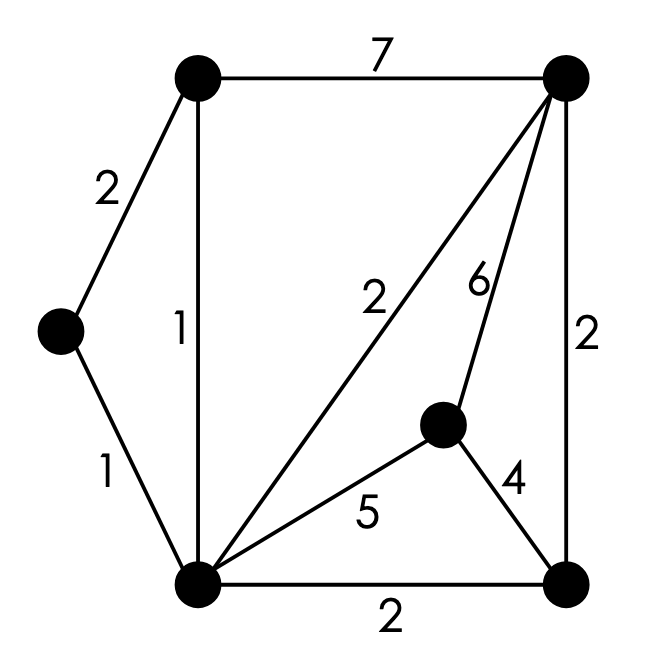
\includegraphics{Bilder/graph_1.png}
		\begin{itemize}
			\item{Der Algorithmus von Kruskal durchsucht global, also muss jede Kante immer beachtet werden.}
			\item{Man kann als erstes eine der beiden Kanten mit Gewicht 1 verwenden. Da diese in beiden Konstellationen keinen Kreis bilden müssen immer beide ausgewählt werden.}
			\item{Es gibt drei Möglichkeiten um die Kante mit Gewicht 2 zu wählen, da eine Möglichkeit einen Kreis bilden würde. Von den drei kann zufällig einer gewählt werden.}
			\item{Unabhängig des Erstgewählten kann ein zweiter ausgewählt werden ohne einen Kreis zu bilden. Der dritte kann jedoch nicht mehr hinzugefügt werden.}
			\item{Die nächste Option ist 4, welche durch die 2 vorherigen Kanten stets gewählt werden mussten. Dieser vollendet den Graphen und es muss nichts mehr hinzugefügt werden.}
		\end{itemize}
		\item[2]{Wenden Sie auf folgenden Graphen den Algorithmus von Prim an um einen minimalen Spannbaum zu ermitteln.}
		%\item{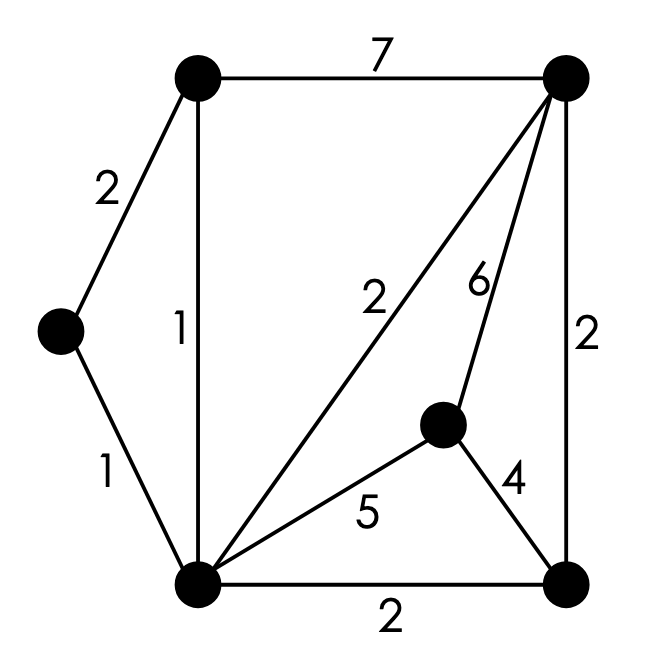
\includegraphics{Bilder/graph_1.png}}
		\begin{itemize}
			\item{Der Algorithmus von Prim durchsucht stattdessen lokal, die Varianz des Spannbaums ist jedoch größer da bei einem zufälligen Knoten begonnen werden kann}
			\item{Wenn mit dem Knoten innerhalb des Dreiecks begonnen wird, kann man nur die Kante mit Gewicht 4 nehmen}
		\end{itemize}

	\end{itemize}




	

	























  
\end{document}